\chapter{Flow around an airfoil at low Reynolds number}
\label{chap-NACA}

\section{Introduction}
\label{sec-C8_introduction}
As noticed at the introduction of this thesis, \Chap{Introduction}, a common application of CFD software is the simulation of flows around airfoils. These simulations are needed by the aerospace industry to optimize their products and reduce the costs of experimentation.

The aim of this chapter is to apply all the numerical improvements that this thesis has contributed with, to the resolution of a realistic problem. We consider the simulation of turbulent incompressible flow around an airfoil, particularly a NACA 0012 airfoil, \cite{NACA}.

The NACA airfoils are widely used as a benchmark of a real life problem, note that many airplane and wind turbines wings are based on these profiles. Both, numerical simulations and experiments in wind tunnels have been done with several configurations of this type of airfoil. The NACA 0012 is one of the mosts used configurations, see for instance \cite{Sheldahl,McCroskey,Rivera}, but other like the NACA 4412 are also widely studied, see \cite{Wadcock 1987 and Hasting and Williams (1984,1987)}. Another type of airfoil that are also used as a benchmark in the literature is the Aerospatiale-A airfoil, used for example in the LESFOIL project \cite{Davidson_2012}.

Although that most of the works that can be found in the literature deal with challenging configurations, i.e. high Reynolds numbers and high angles of attack, see \cite{jansen_stabilized_1999, kaltenbach_large-eddy_1995, schmidt_assessment_????,lesons_from_LESFOIL}, we will restrict ourself to a more modest scenario. That is to consider low Reynolds number with moderate angles of attack. The main reason for considering this case is the possibility to compare the results obtained with a weak treatment of the Dirichlet boundary conditions against the obtained with a strong imposition of the Dirichlet boundaries, without the need of spending too many computational resources.

Nevertheless, the simulation of turbulent flow around an airfoil at low Reynolds number is gaining interest in the recent years. This increase on the demand of the simulation of such flows is caused by the fact that aircraft-like devices have been proposed as possible Mars explorers, see \cite{Kojima,smith_2003,anyoji_2010}. These vehicles are being designed to take photographs of Mars while traveling at low-speed in a thin atmosphere, resulting in a low Reynolds number ($ 10^3\le Re\le10^5 $) environment.

In this type of problems the mesh design plays an important role on the solution, in particular, a proper spacing has to be used at the boundary layer. If a strong definition of the Dirichlet boundary conditions is considered, we say that the simulation is a \textit{Wall-Resolved LES} (WRLES). According to \cite{piomelli_large-eddy_1996}, the coherent structures that appear in the turbulent boundary layer can be captured with a WRLES method if the near-wall node of the mesh is located at a wall distance $y^+<2$ and the streamwise cell size is within the range $50<\Delta x^+<150$. Otherwise, when a wall-law model is used considering weak imposition of the Dirichlet boundary conditions, we say that the simulation is a \textit{Wall-Modeled LES} (WMLES).

In this chapter we will consider the SVMS approach, described in \Chap{SVMS}, considering the weak imposition of Dirichlet boundary conditions. Our concern is to check the feasibility of the proposed method as a WMLES method for the simulation of turbulent flows around an aircraft. In such simulations many flow characteristics are stressed, dealing not simply with turbulent flows, but also with other difficulties like the presence of very thin laminar boundary layers, transition from laminar to turbulent regimes, wall-bounded flow or flow that separates from curved surfaces. The fact is that LES methods have been shown to be very useful for flows where the turbulent structure is dominated by the large-scale structures, like the TGV test discussed in sections \ref{subsec:TGV-VMS} and \ref{subsec:TGV-SRK} or homogeneous turbulent problems, see \cite{colomes_2014}. Despite that, the simulation of near-wall flows using LES methods has demonstrated to be a challenging task, manly because of the complex physical phenomena like the reduction of the large scales structures near the wall, the flow anisotropy or the mesh sensitivity to high aspect ratios. 

Many works have been done discussing the suitability of LES methods for the simulation of flow around an airfoil. This is the case of the European project LESFOIL \cite{davidson_lesfoil:_2003}, where nine different academic and industrial groups worked with the aim to identify the potential of LES as a prediction method for separation in high-Reynolds-number airfoil flows. In this case, the simulated geometry was the Aerospatiale-A airfoil operating at a chord Reynolds number equal to $2.1\cdot10^6$ with an angle of attack equal to $13.3^o$ and a Mach number of $0.15$. Other authors have been worked with NACA type airfoils. This is the case of \cite{jansen_stabilized_1999, kaltenbach_large-eddy_1995, schmidt_assessment_????}, where the use of LES method for the simulation of the flow around a NACA4412 airfoil is studied using unstructured, structured and semi-structured grids, respectively.

This chapter is structured as follows ...

%The simulation of this test is done on a structured mesh around the airfoil profile and unstructured mesh on the remaining domain, see Fig. \ref{fig-NACA_mesh_global}, which allow us to have fine enough elements around the airfoil surface, the turbulent boundary layer and the wake region, while coarse elements are used in the far field region. At the leading edge, the near wall-node is located at $y\sim 2.0\cdot10^{-5}c$ which leads to a wall distance of $ y^+\sim1.4$. This distance is kept almost constant at the laminar region and is increased constantly until it reaches the maximum of $y\sim1.0\cdot10^{-4}$ at the trailing edge, where the wall distance is less restrictive $y^+<1$. The spanwise elemental length is $\Delta x\sim0.0015c$ constant over all the suction side of the airfoil, which at the leading edge give a normalized distance of $\Delta x\sim105$. We see that the mesh sizes satisfy the conditions needed to capture the boundary layer phenomena.
%
%Let us now consider the simulation of the flow around an airfoil near maximum lift. In particular, we select a NACA 4412 airfoil under a flow with an angle of attack of $12^o$, which, according to Wadcock 1987 and Hasting and Williams (1984,1987), was determined to be the one that results in the maximum lift.

\section{Problem statement}
\label{sec-C8_prob_statement}

Let us briefly review the statement of the problem that will be studied in this chapter. Let $\Omega$ be a bounded domain of $\mathbb{R}^d$, where $d=2,3$ is the number of space dimensions, $\Gamma=\partial\Omega$ its boundary and $(0,T]$ the time interval. The strong form of the transient Navier-Stokes problem consists in finding the velocity field $\u$ and the pressure field $p$ such that 
\begin{align}
\label{eq-C8_NS_strong_mome}
\partial_t\u-\nu\Delta\u+\u\cdot\nabla\u+\nabla p&=\f&\mbox{in $\Omega\times(0,T]$,}\\
\label{eq-C8_NS_strong_inc}
\nabla\cdot\u&=0&\mbox{in $\Omega\times(0,T]$,}
\end{align}
with $\f$ being the force vector and $\nu$ the kinematic viscosity. Equations \Eq{C8_NS_strong_mome} and \Eq{C8_NS_strong_inc} are supplied with appropriate boundary and initial conditions, as stated in \Eq{NS_strong_Dir}-\Eq{NS_strong_Ini}.

From equations \Eq{C8_NS_strong_mome}-\Eq{C8_NS_strong_Ini} one can derive the weak form of the problem, which consists in finding $[\u,p]\in\mathbf{L}^2(0,T;\mathcal{V}_g)\times L^1(0,T;\mathcal{Q}_0)$ such that
\begin{equation}
\label{eq-C8_NS_weak}
(\partial_t\u,\v)+B(\u,(\u,p),(\v,q)) = \left<\f,\v\right> 
\quad\quad\forall\v\in\mathcal{V}_0,\quad\forall q\in\mathcal{Q}_0,
\end{equation}
satisfying the initial condition \Eq{NS_strong_Ini} in a weak sense. Here $\mathcal{V}_0:=\mathbf{H}_0^1(\Omega)$, $\mathcal{V}_g:=\mathbf{H}_g^1(\Omega)$  and $\mathcal{Q}_0:=L^2(\Omega)/\mathbb{R}$ and the form $B(\u,(\u,p),(\v,q))$ is defined as 
\begin{equation}
\label{eq-C8_bilinear}
B(\u,(\u,p),(\v,q)):=\nu(\nabla\u,\nabla\v)+b(\u,\u,\v)-(p,\nabla\cdot\v)+(q,\nabla\cdot\u)
\end{equation}

Let us consider a FE partition $\mathcal{T}_h$ of the domain $\Omega$ from which we can construct conforming finite dimensional spaces for the velocity $\mathcal{V}_{0,h} \subset \mathcal{V}_0$, $\mathcal{V}_{g,h} \subset \mathcal{V}_g$, and for the pressure $\mathcal{Q}_{0,h}\subset \mathcal{Q}_0$. Let us also consider the VMS decomposition (see \Sec{C2_vms}) $\mathcal{V}_0=\mathcal{V}_{0,h}\oplus\widetilde{\mathcal{V}}_0$, $\mathcal{V}_g=\mathcal{V}_{g,h}\oplus\widetilde{\mathcal{V}}_g$ and $\mathcal{Q}=\mathcal{Q}_{0,h}\oplus\widetilde{\mathcal{Q}}_0$, where $\widetilde{\mathcal{V}}_0$, $\widetilde{\mathcal{V}}_g$ and $\widetilde{\mathcal{Q}}_0$ are infinite-dimensional spaces that complete the FE spaces in $\mathcal{V}_0$, $\mathcal{V}_g$ and $\mathcal{Q}_0$, respectively.

From the weak form of the Navier-Stokes equations \Eq{C8_NS_weak}-\Eq{C8_bilinear}, and following the approach of a mixed FE formulation with convection stabilization through an OSS method, described in \Chap{TBT_OSS}, we can derive the semi-discrete form as follows
\begin{equation}
\label{eq-C8_NS_discrete}
(\partial_t\u_h,\v_h)+B_{tbt\_oss\_iss}(\u_h,(\u_h,p_h),(\v_h,q_h)) =L_h(\v_h,q_h)\quad\quad\forall\v_h\in\mathcal{V}_{0,h},\forall q_h\in\mathcal{Q}_{0,h},
\end{equation}
with $L_h(\v_h,q_h)=\left<\f,\v_h\right>$  and
\begin{align}
\label{eq-C8_biliniar_oss_tbt_iss}
B_{tbt\_oss\_iss}(\u_h,(\u_h,p_h),(\v_h,q_h))&=B_h(\u_h,(\u_h,p_h),(\v_h,q_h))\\\nonumber
&+(\tau_m\u_h\cdot\nabla\u_h,\u_h\cdot\nabla\v_h)-(\tau_m\etaa_h,\u_h\cdot\nabla\v_h)\\\nonumber
&+(\tau_c\nabla\cdot\u_h,\nabla\cdot\v_h)
\end{align}
being
\begin{equation}
\label{eq-C8_bilinear_discrete}
B_h(\u_h,(\u_h,p_h),(\v_h,q_h)):=\nu(\nabla\u_h,\nabla\v_h)+b(\u_h,\u_h,\v_h)-(p_h,\nabla\cdot\v_h)+(q_h,\nabla\cdot\u_h).
\end{equation}
The convective term $ b(\u_h,\u_h,\v_h) $ is defined with the skewsymmetric version exposed in \Eq{C2_b_skew1}. In \Eq{C8_biliniar_oss_tbt_iss}, the unknown $ \etaa_h $ stands for the projection of the convective term into the FE space, computed as follows
\begin{align}
\label{eq-C8_NSprojectiondef1}
&(\tau_m\etaa_h,\kppa_h) = (\tau_m \u_h\cdot\nabla\u_h,\kppa_h)&\forall \kppa_h\in\mathcal{V}_{h,0},
\end{align}
with the expressions of the stabilization parameters $\tau_m$ and $\tau_c$ being
\begin{align}
\label{eq-C8_tau_m}
&\tau_m=\left(\frac{c_1\nu}{h^2}+\frac{c_2|\a|}{h}\right)^{-1},\\
\label{eq-C8_tau_c_alt}
&\tau_c=c_c\left(\nu+\frac{c_1}{c_2}h|\u_h|\right),
\end{align}
where $h$ is the characteristic mesh size and $c_1$, $c_2$ and $ c_c $ are algorithmic constants, see \Sec{C2_vms} for a deeper description of the origin of these parameters.

As explained in the introduction of this chapter, the main purpose here is to assess the feasibility of the SVMS method with weak Dirichlet boundary conditions as a WMLES model for the simulation of a flow around an airfoil. Then we will make use of the formulation defined in Section \ref{subsec-C7_weak_bcs} for the weak imposition of the Dirichlet boundary conditions, which can be summarized considering the following biliniar form instead of \Eq{C8_biliniar_oss_tbt_iss}
\begin{align}
\label{eq-C8_bilinear_weak_by_components}
B_{weak}(\u_h,(\u_h,p_h),(\v_h,q_h))&=B_\Gamma(\u_h,(\u_h,p_h),(\v_h,q_h))\\\nonumber
&+\left(\alpha_{b,n}(\u_h-\u_g),(\n\otimes\n)\v_h\right)_{\Gamma_D}\\\nonumber
&+\left(\alpha_{b,\tau}(\u_h-\u_g),(\boldI-\n\otimes\n)\v_h\right)_{\Gamma_D}\\\nonumber
&-((\u_h-\u_g),(q_h\mathbf{I}+2\nu\nabla^s\v_h)\cdot\n)_{\Gamma_D}.
\end{align}
where $ B_\Gamma(\u,(\u,p),(\v,q)) $ is equivalent to the definition \Eq{C8_biliniar_oss_tbt_iss} when the terms that appear on the boundary are considered, see \Eq{C7_bilinear_boundary}. These terms arise when we extend the space of the FE functions from $ \v_h\in\mathcal{V}_{0,h} $ to $ \v_h\in\mathcal{V}_h $. Furthermore, $ \alpha_{b,n} $ and $ \alpha_{b,\tau} $ are the penalty constants for the wall-normal and tangential components, respectively, which definition can be found in equations \Eq{C7_alpha_b_n}-\Eq{C7_alpha_b_t}.

\section{Test setting}
\label{sec-C8_setting}
In this test we study the flow around a NACA 0012 airfoil with a span-wise length of $ 0.16c $, being $ c $ the chord length. In \Fig{NACA_geometry} we depict the geometry of the studied airfoil.
\begin{figure}[h!]
  \centering
  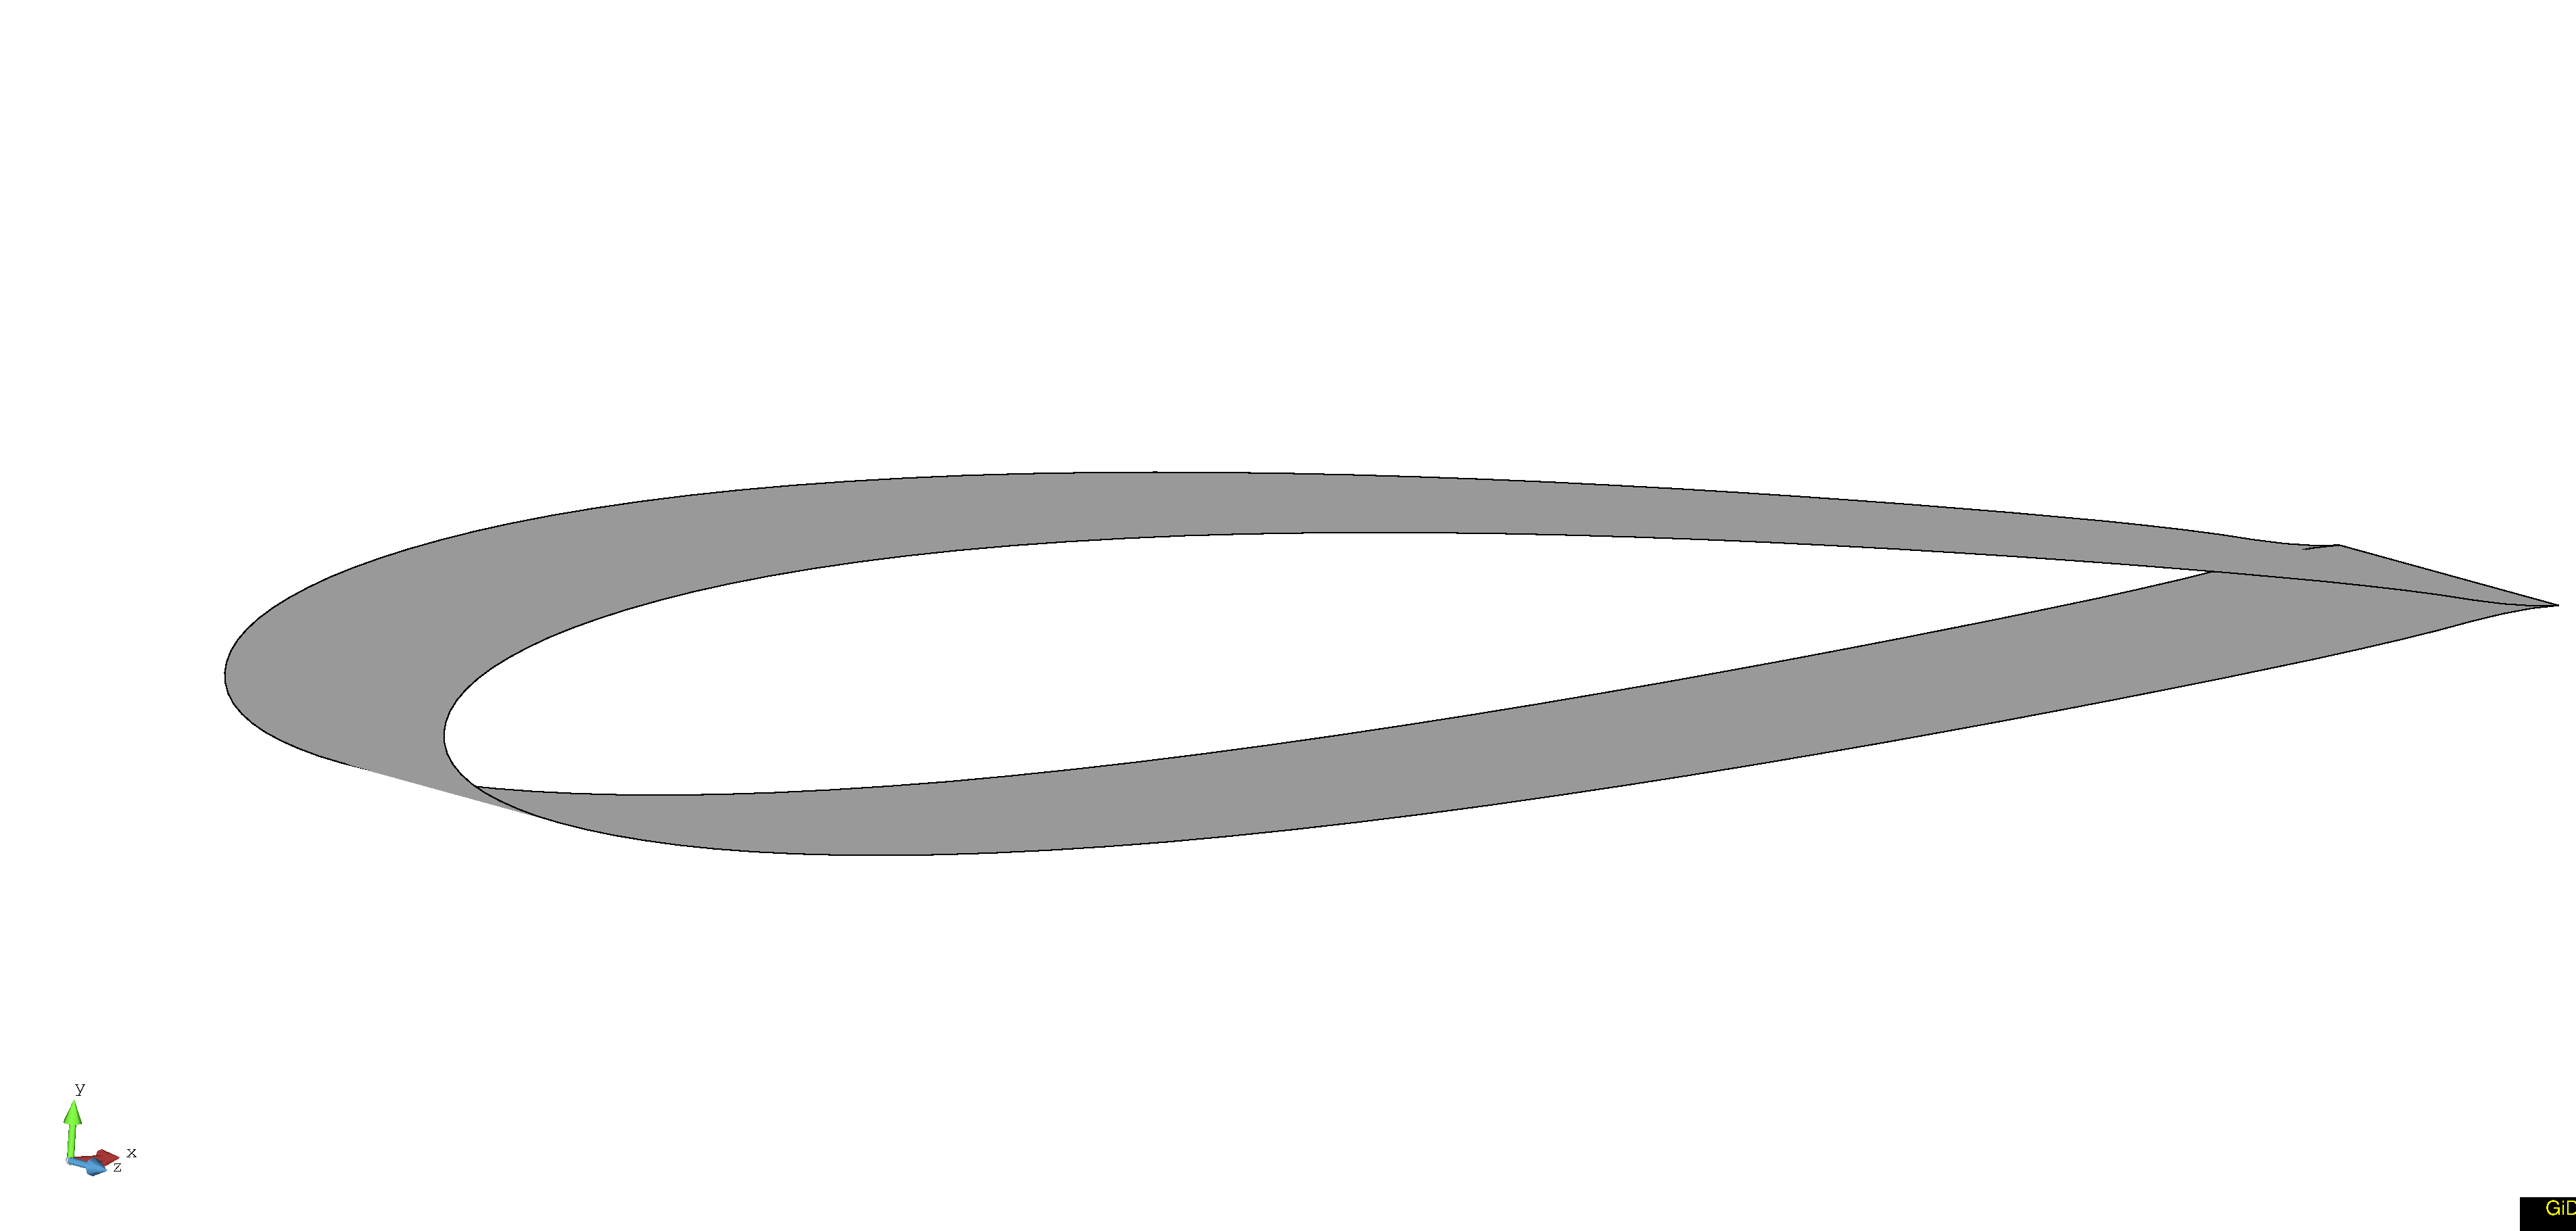
\includegraphics[width=0.7\textwidth,clip=true,trim=5cm 8cm 1cm 8cm]{Figures/Chapter8/geometry_3d}
  \caption{NACA 0012 airfoil geometry.}
  \label{fig-NACA_geometry}
\end{figure}
The computational domain is defined with an inlet and outlet boundaries around 10 chord lengths away from the airfoil surface. At the inlet boundary a freestream velocity $U_\infty=10$ has been setted, while the outlet boundary has left free. We consider an angle of attack of $ \alpha = 6 $ deg and a Reynolds number based on the chord length $ Re_c=2.3\cdot10^4 $, the same used in \cite{kojima,kim}.

The simulation of this test is done on a structured C-type mesh around the airfoil profile. We consider two different 2-dimensional meshes of quadrilaterals, one much finner than the other, that are extruded along the span-wise direction. The goal of using two different meshes is to assess the performance of the weak imposition of the Dirichlet boundary conditions at the airfoil surface. We define the meshes in a such way that we have fine enough elements around the airfoil surface, the turbulent boundary layer and the wake region, while coarse elements are used in the far field region. In \Fig{NACA_meshes} we depict the two meshes used in this test.
\begin{figure}[h!]
  \centering
  \subfigure[Coarse mesh.]{\label{fig-NACA_mesh_coarse}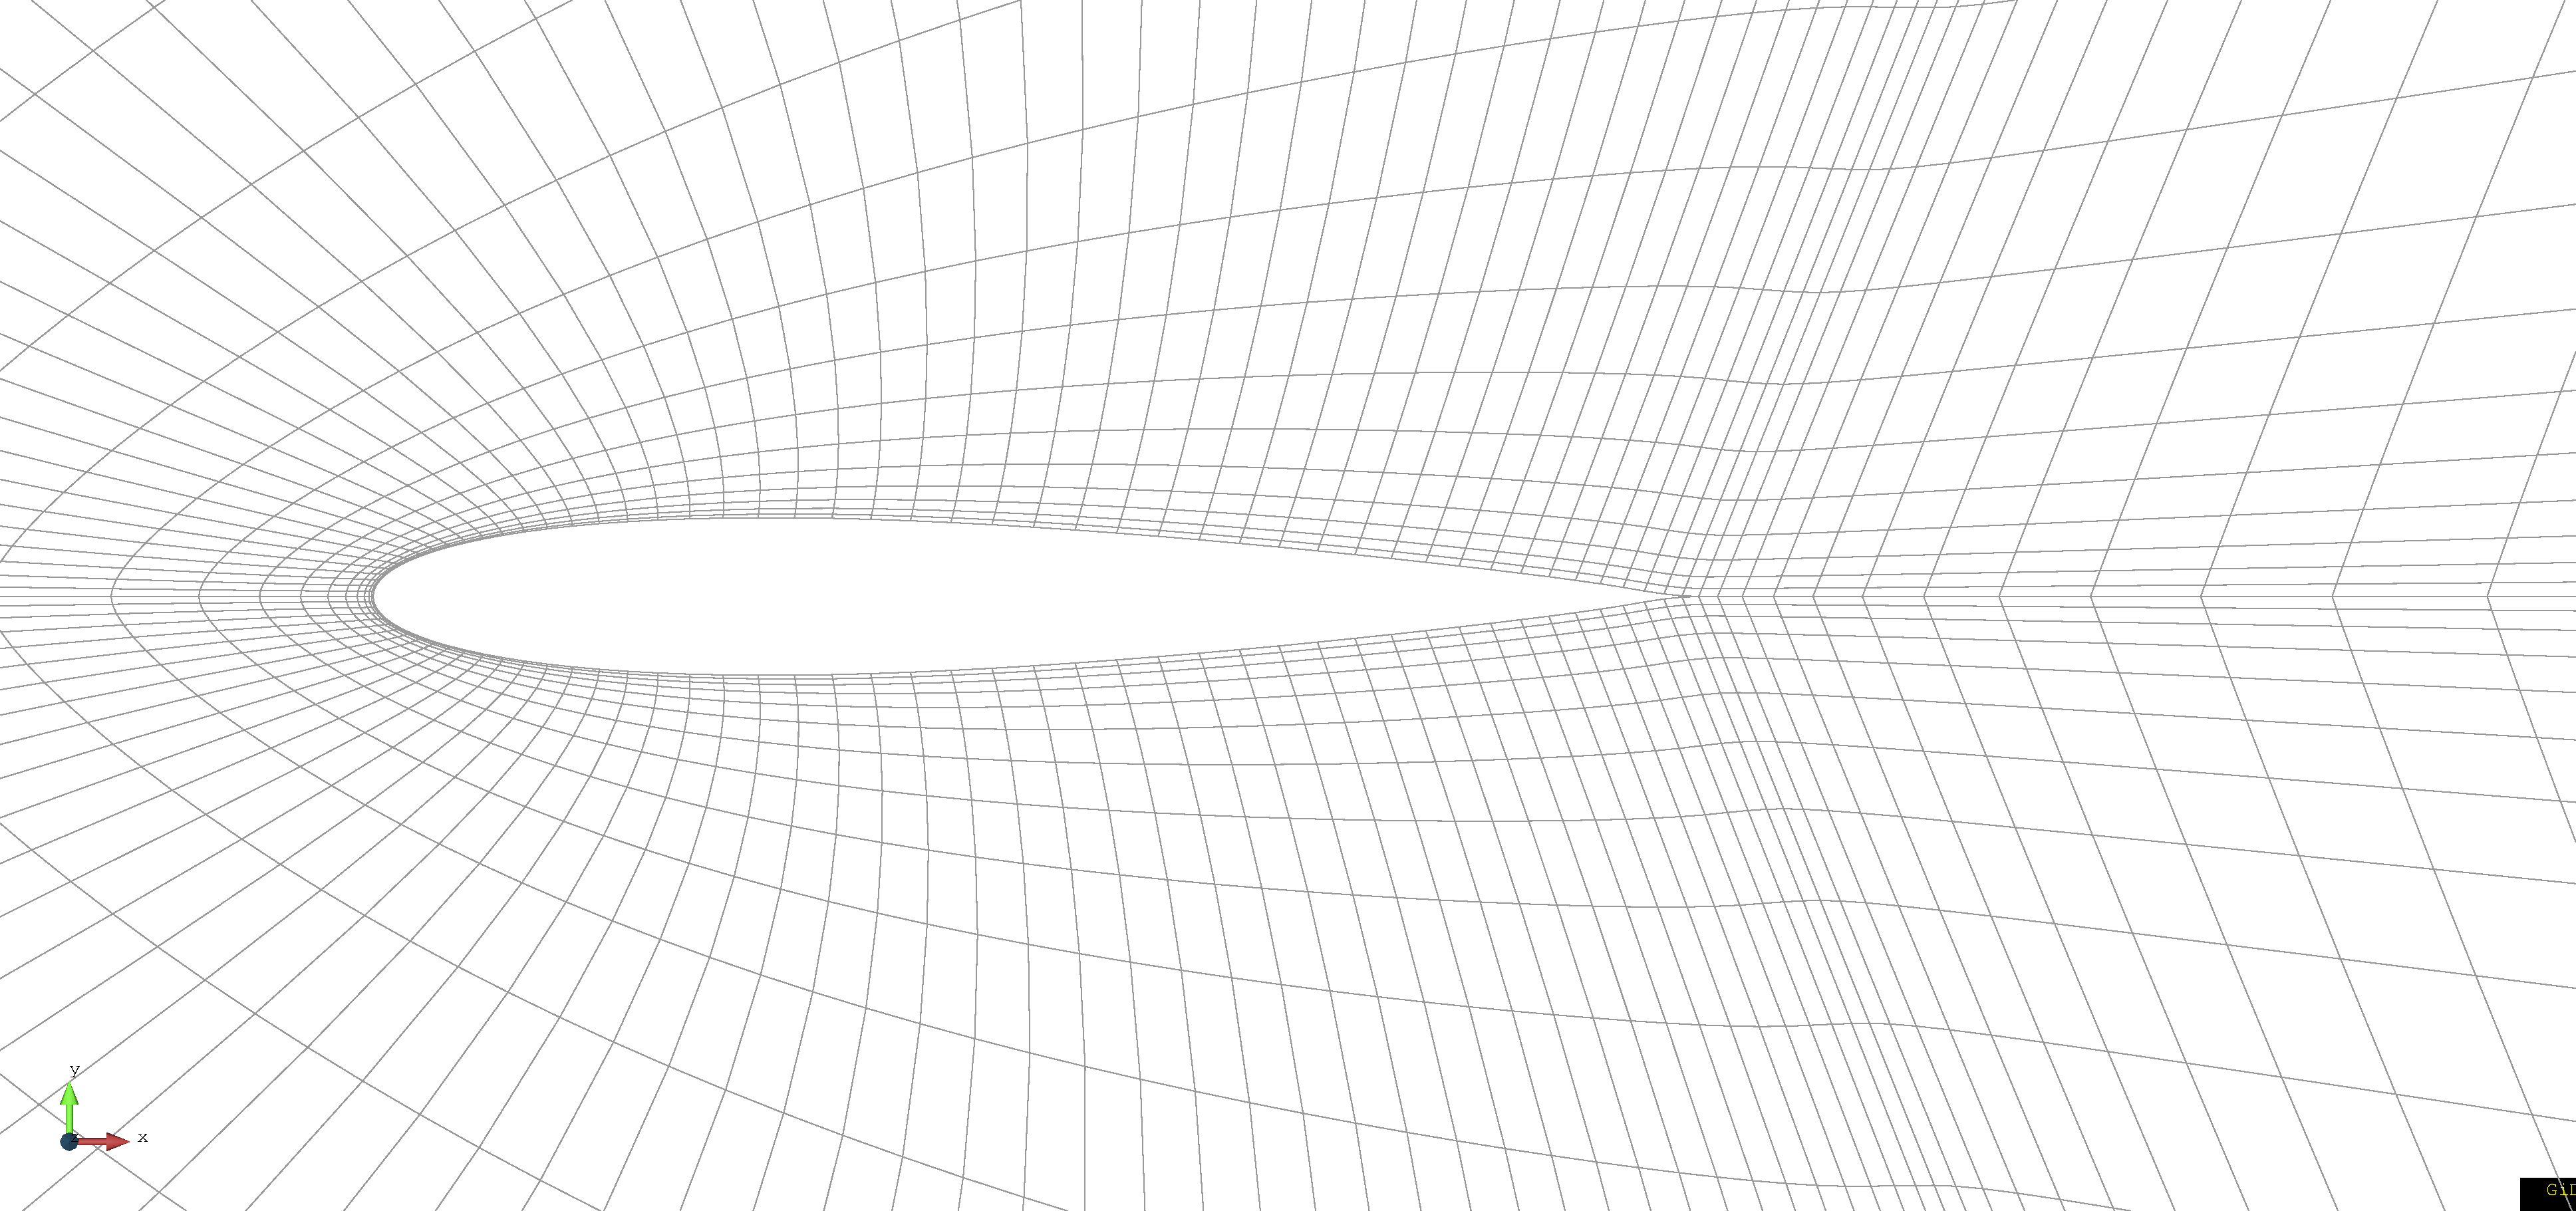
\includegraphics[width=0.7\textwidth]{Figures/Chapter8/mesh_coarse}}\\
  \subfigure[Close up view of the fine mesh.]{\label{fig-NACA_mesh_fine_close}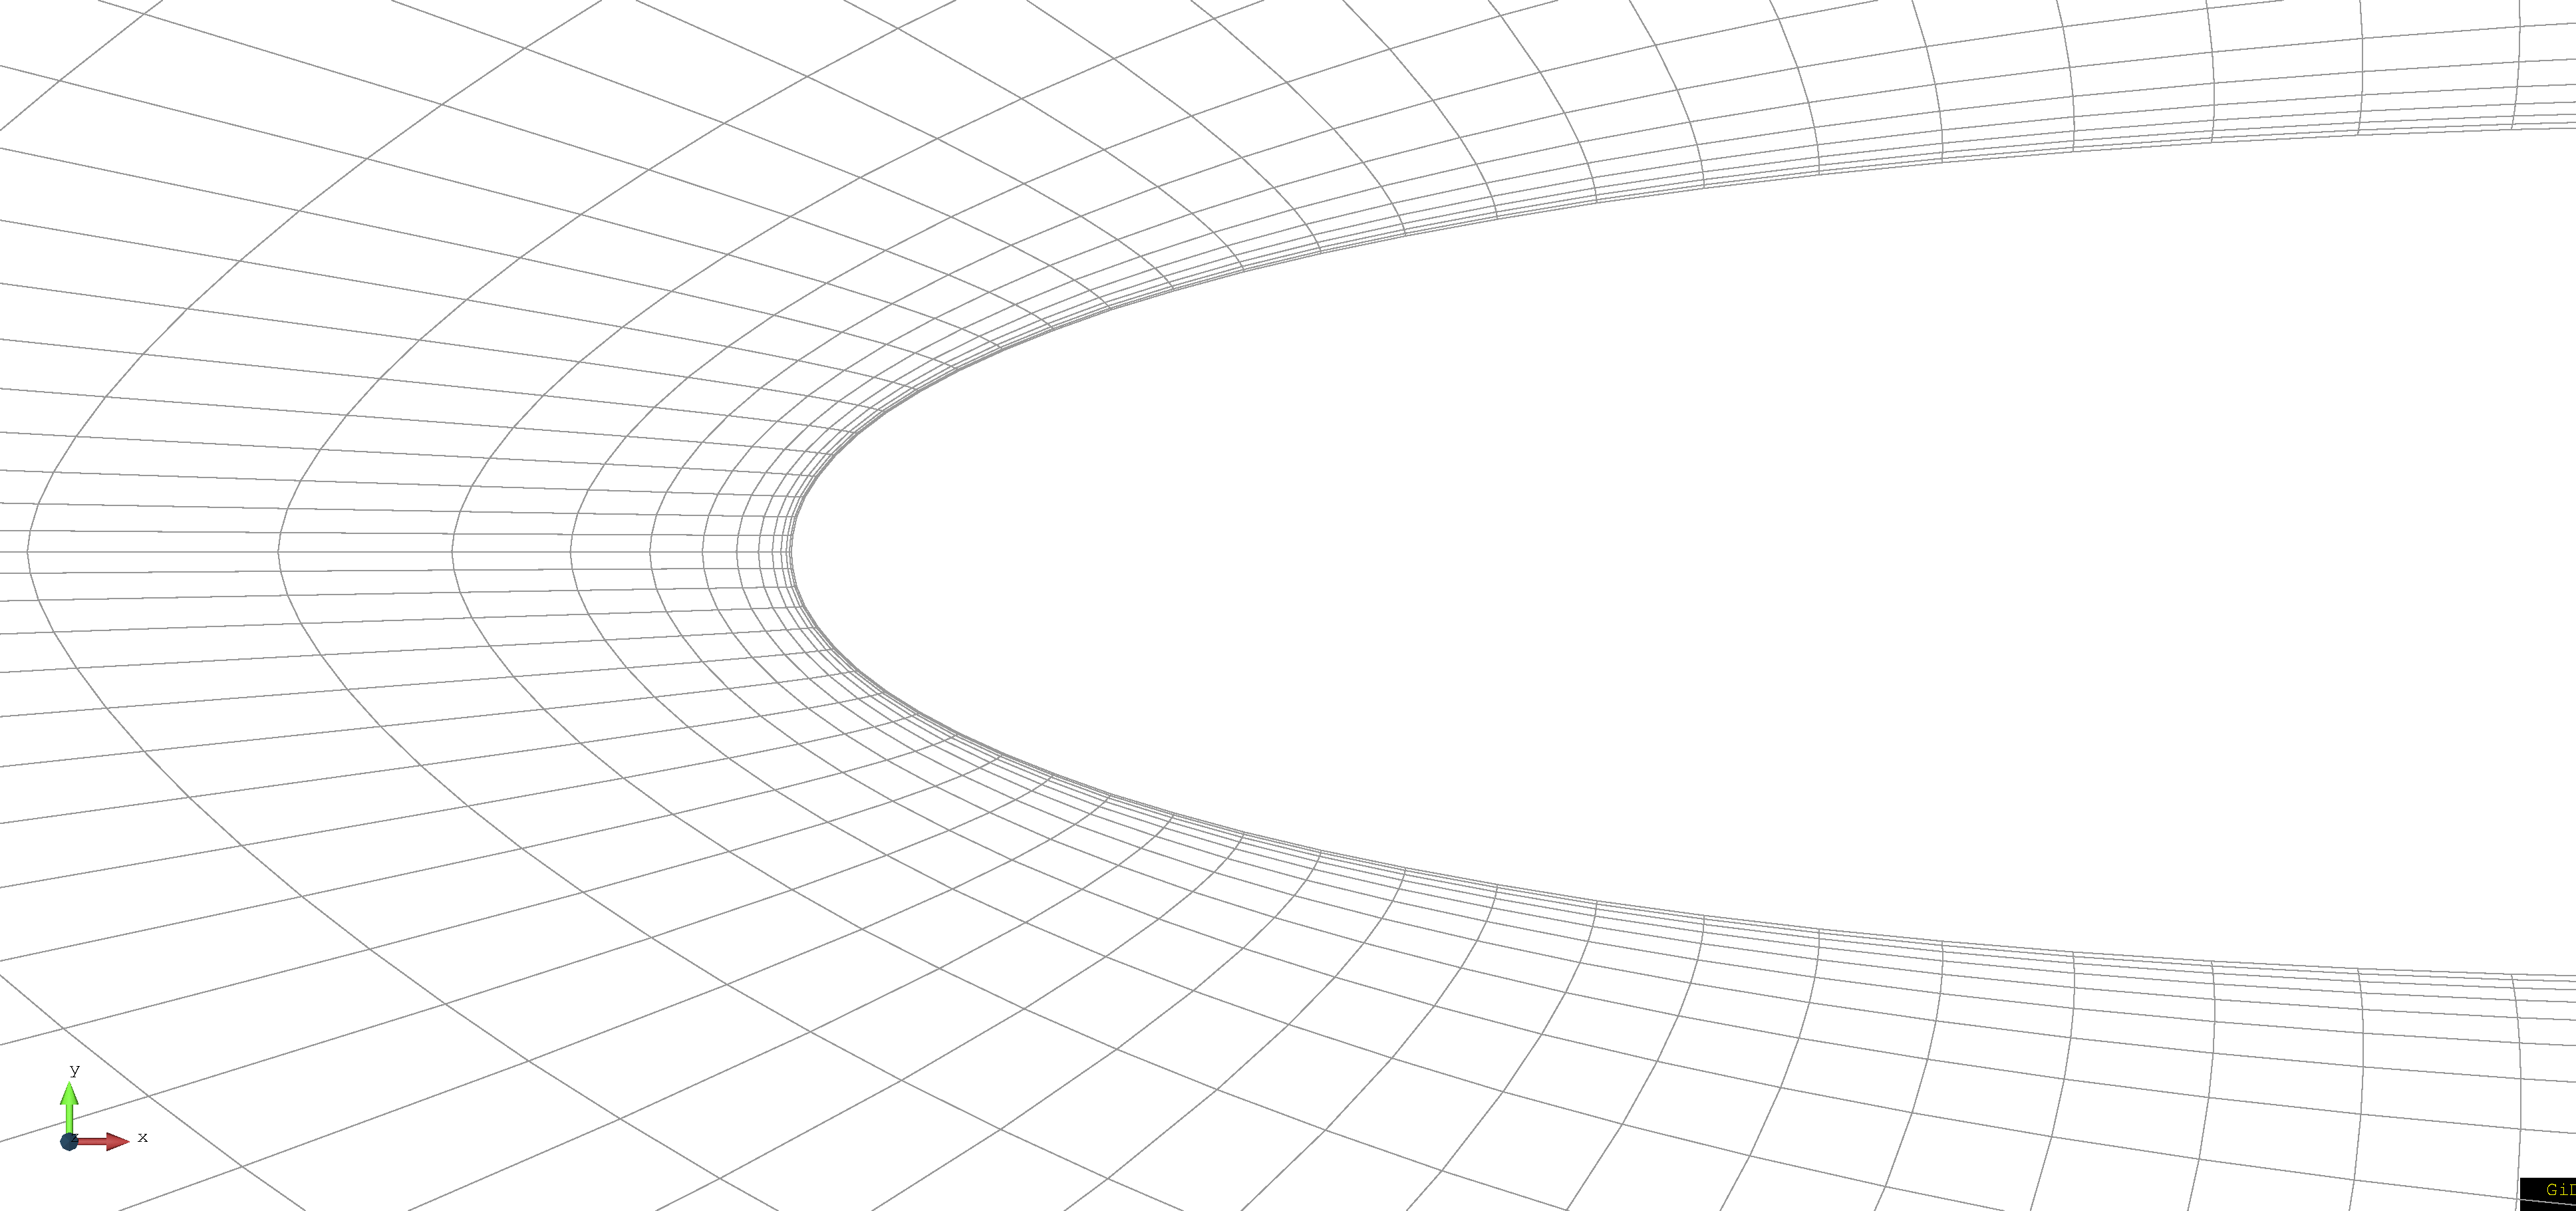
\includegraphics[width=0.7\textwidth,clip=true,trim=8cm 2cm 10cm 2cm]{Figures/Chapter8/mesh_fine_close}}\\
  \subfigure[Close up view of the coarse mesh.]{\label{fig-NACA_mesh_coarse_close}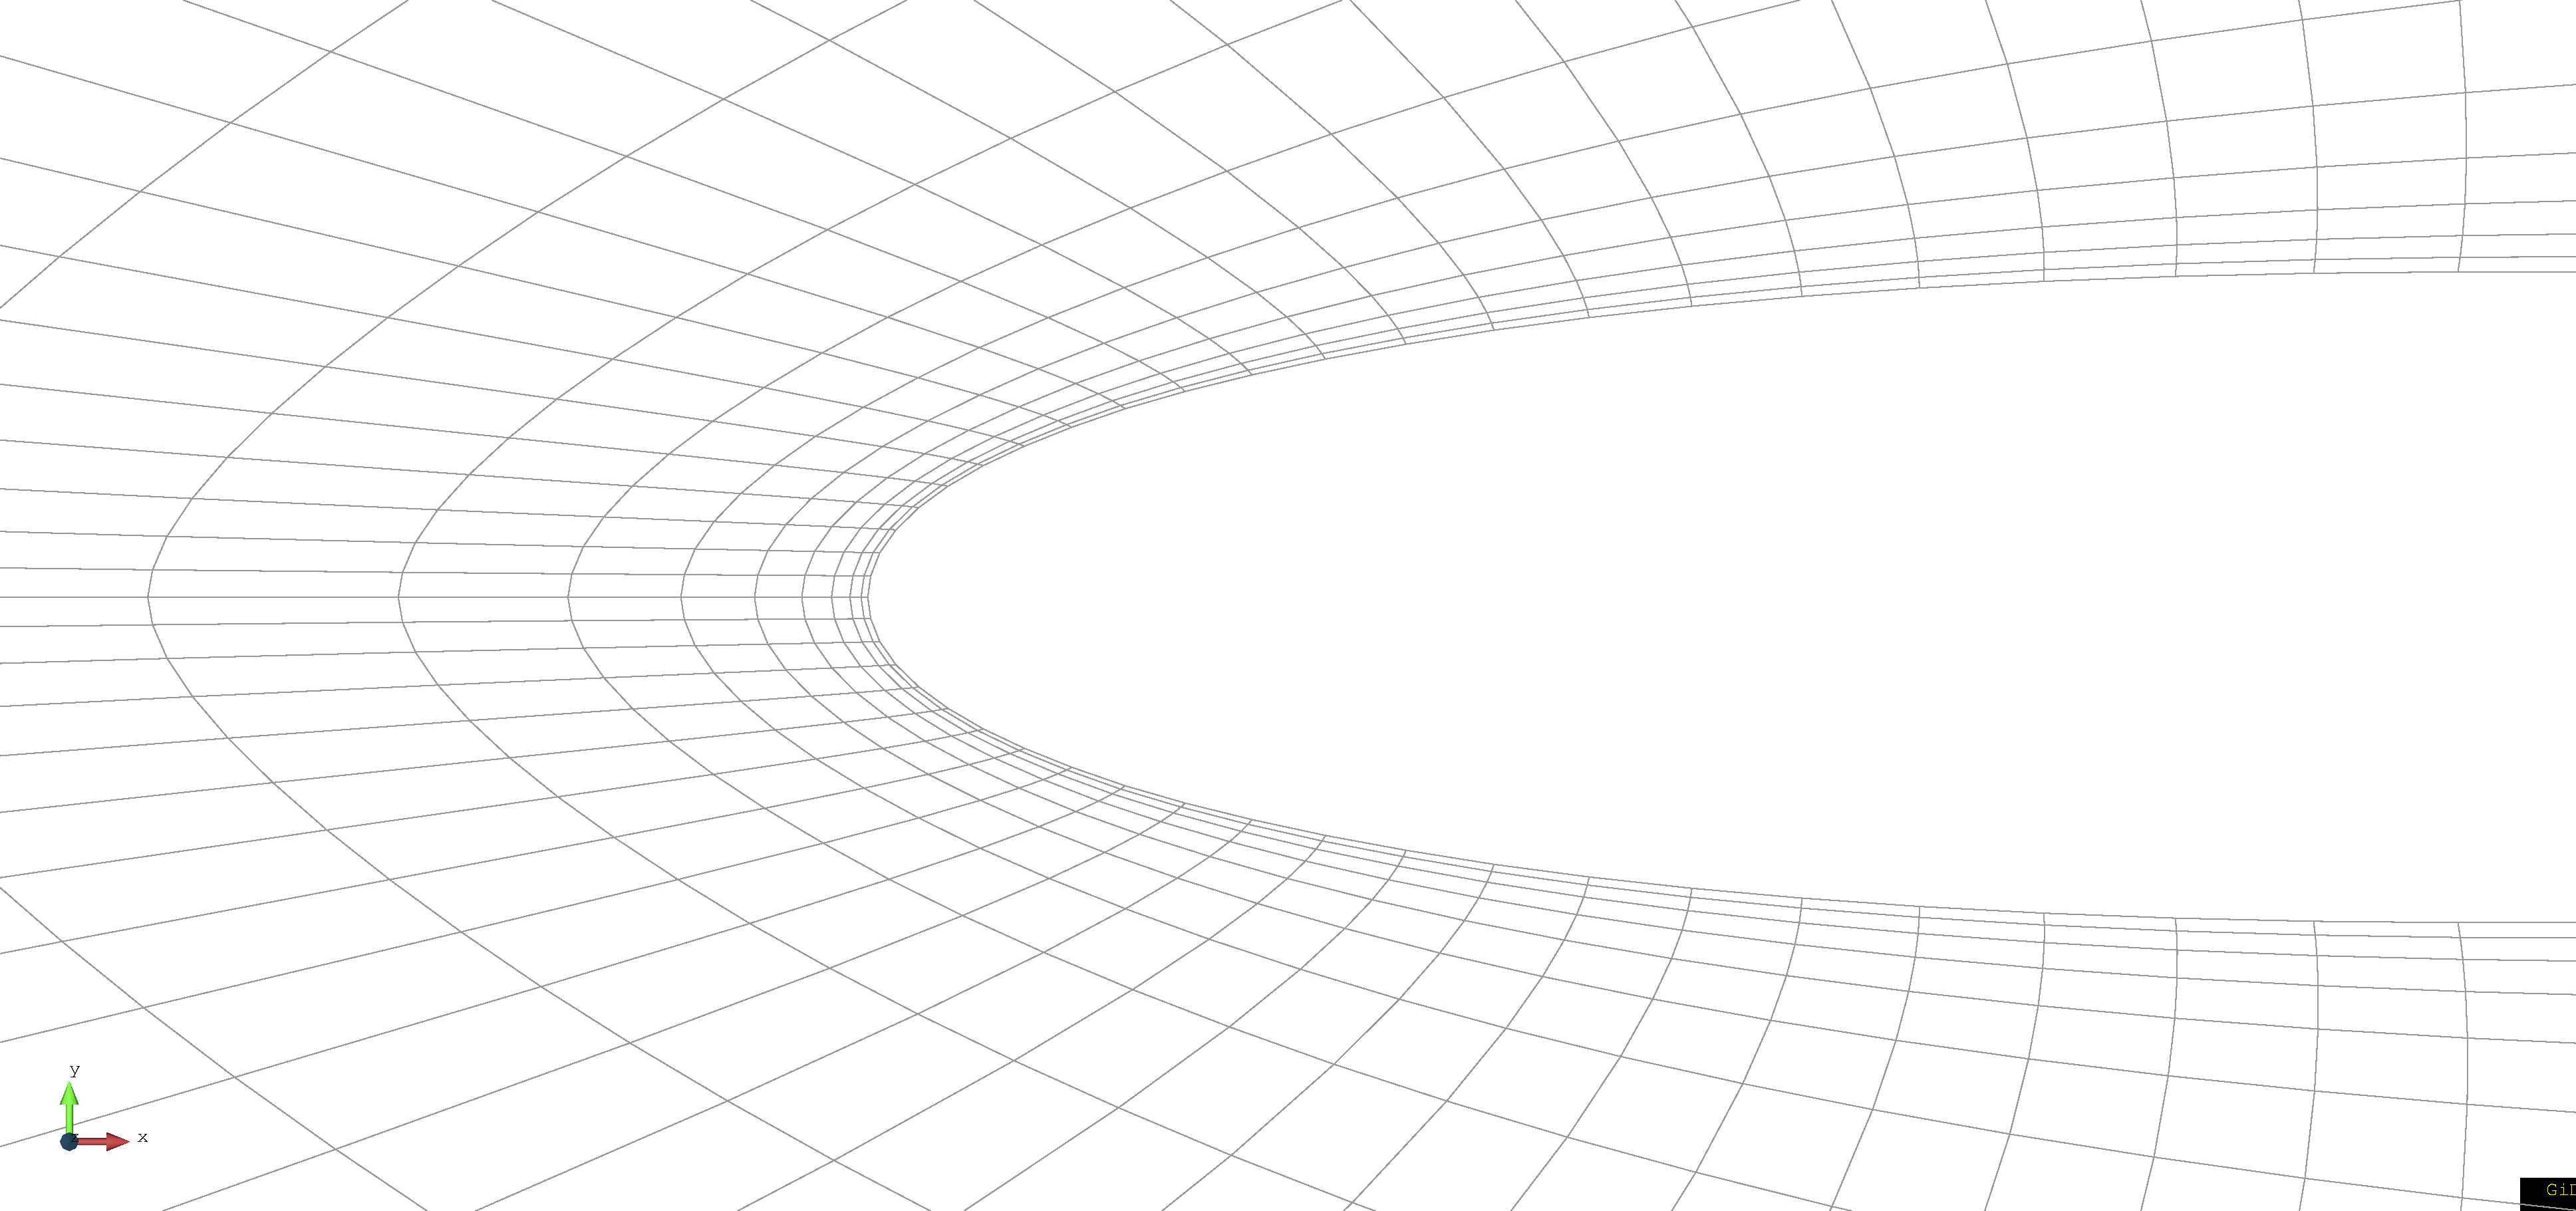
\includegraphics[width=0.7\textwidth,clip=true,trim=12cm 6cm 18cm 6cm]{Figures/Chapter8/mesh_coarse_close}}
  \caption{NACA 0012 meshes.}
  \label{fig-NACA_meshes}
\end{figure}
Focusing on the finner mesh, shown in \Fig{NACA_mesh_fine_close}, at the leading edge, the near wall-node is located at $y\sim 2.0\cdot10^{-4}c$ which leads to a wall distance of $ y^+<1$. This distance is kept almost constant at the laminar region and it is increased constantly until it reaches the maximum of $y\sim2.0\cdot10^{-3}$ at the trailing edge, where the wall distance is less restrictive. The maximum stream-wise elemental length is $\Delta x\sim0.028c$ located at the suction side of the airfoil, giving a normalized distance of $\Delta x^+\sim40$. We see that the mesh sizes satisfy the conditions needed to capture the boundary layer phenomena.

Regarding the coarse mesh, see \Fig{NACA_mesh_coarse} and \Fig{NACA_mesh_coarse_close}, the near wall-node is located at $y\sim 1.2\cdot10^{-3}c$ leading to a wall distans of the order of $ y^+\sim 2 $. This distance is constantly increased until it reaches a value of $y\sim6.4\cdot10^{-3}c$ at the trailing edge, much grater than the finner mesh. In this mesh, the maximum stream-wise elemental length is $\Delta x\sim0.032c$ that is equivalent to a normalized distance of $\Delta x^+\sim50$. We only compute the 3D test on the coarse mesh, with a constant span-wise elemental length equal to $ \Delta z\sim0.02c $.

The spatial discretization is done using inf-sup stable elements $Q_2/Q_1$. These type of elements will allow us to use the SVMS approach descrived in the previous \Sec{C8_prob_statement}. Here we use the same algorithmic parameters, $ c_1=12.0 $ and $ c_2=8.0, $ as used in Section \ref. The problem is solved using the IMEX version of the SRK method introduced in \Chap{SRK} and also used in \Chap{SVMS} with a \textit{(3-3)} scheme, see Appendix \ref{appendix-SRK}, and an adaptive time stepping technique as exposed in Section \ref{subsec-C7_adaptive}. The time step size evolves tending to $ \delta t= 5.0\cdot10^{-4}c/U_\infty$ giving a maximum hyperbolic CFL around $ 0.3 $.

\section{Simulation results and discussion}
\label{sec-C8_results}
In order to check the suitability of the proposed methods we start with a 2-dimensional simulation comparing the results obtained with the fine and coarse meshes. For such computations, we begin with an initial solution that has been computed solving the Stokes problem. We solve the problem from $ t=0.0 $ to $ t=1.0 $ wich is equivalent to $ 10 $ time units ($1$ time unit $=c/U_\infty$).

\subsection{Effect of $ c_c $ in a 2D mesh with strong BCs}
We first analyse the effect of the $ c_c $ constant that appear in equation \Eq{C8_tau_c_alt}. We know by the experience acquired on the turbulent tests performed in \Chap{TBT_OSS} and \Chap{SVMS} that this parameter plays a relevant role when inf-sup stable elements are used. Here we choose the set of values $ c_c = \{1.0,2.0,4.0,8.0,16.0,32.0\} $ and solve the problem from $ t=0.0 $ to $ t=1.0 $ using the finner mesh with strong boundary conditions.

We depict the Drag and Lift coefficients in \Fig{NACA_c_c_drag_lift}, computed as stated in Section \ref{subsec-C6_cylinder}. It is seen in both the drag (\Fig{NACA_c_c_drag}) and lift (\Fig{NACA_c_c_lift}) coefficients that at some point, the computations for $ c_c<32.0 $ blows up.
\begin{figure}[h!]
  \centering
  \subfigure[Drag coefficient.]{\label{fig-NACA_c_c_drag}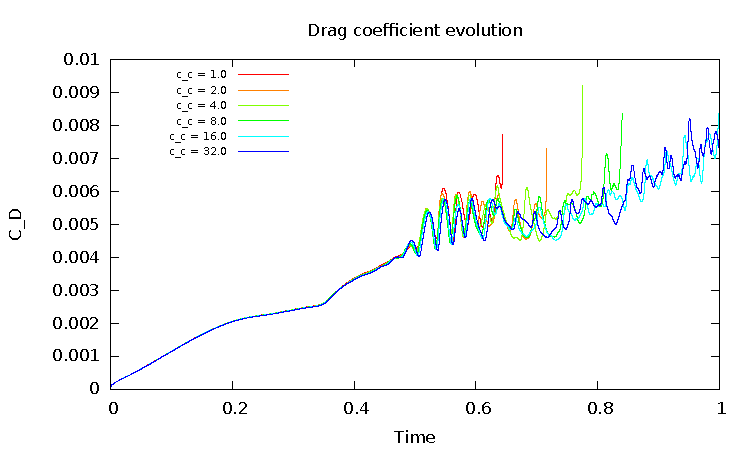
\includegraphics[width=0.6\textwidth]{Figures/Chapter8/strong/drag}}\\
  \subfigure[Lift coefficient.]{\label{fig-NACA_c_c_lift}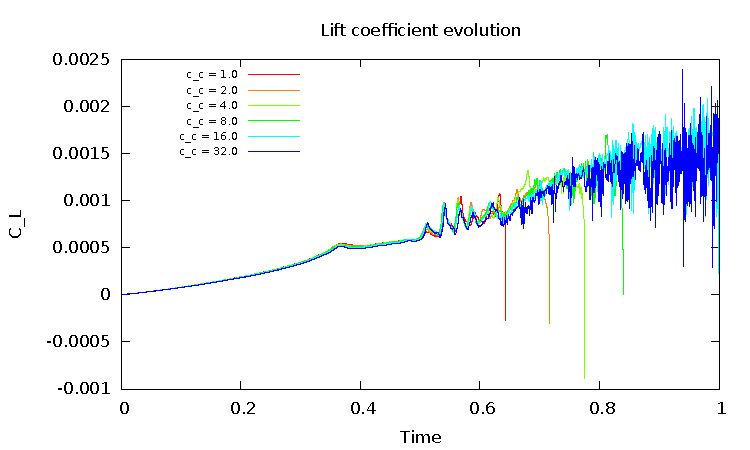
\includegraphics[width=0.6\textwidth]{Figures/Chapter8/strong/lift}}
  \caption{Drag and Lift coefficients for the 2D computation for different $ c_c $ values.}
  \label{fig-NACA_c_c_drag_lift}
\end{figure}
Let us now focus on the evolution of the velocity divergence norm, which is shown in \Fig{NACA_c_c_divel} scaled by the kinetic energy of the problem. It is seen on this figure that, for $ c_c<32.0 $, the velocity divergence norm is increased with a constant rate until it reaches an unstable point from wich it explodes. This behavior does not occur for $ c_c=32.0 $ until $ t=1.0 $. We also see that the rate of increase of the velocity divergence tends to the one followed by the $ c_c=32.0 $ case. This constant increase shown in \Fig{NACA_c_c_divel} is normal and may be caused by the flow development from a laminar initial solution to a fully developed turbulent flow.
\begin{figure}[h!]
  \centering
  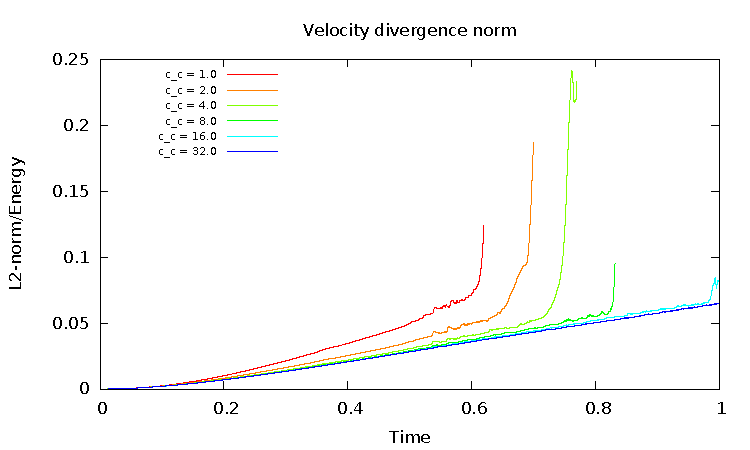
\includegraphics[width=0.6\textwidth]{Figures/Chapter8/strong/divel}
  \caption{$\|\nabla\cdot\u\|/K$ for the 2D computation for different $ c_c $ values.}
  \label{fig-NACA_c_c_divel}
\end{figure}
In the forthcomming computations of this test we will use $ c_c=32.0 $.

\subsection{Effect of $ \beta $ in a 2D mesh with weak BCs}
Once analysed the effect of the constant $ c_c $ on the solution, we proceed to check the effect of the $ \beta $ constant that appear on the definition of the weak imposition of the wall-normal component on the Dirichlet boundary. In this case we select four different values, $ \beta={10,100,1000} $ and we solve the problem on the coarse mesh from $ t=0.0 $ to $ t=0.5 $.

In this case, as it is seen in \Fig{NACA_b_drag_lift}, any difference can be distinguished during the laminar transition to turbulent flow for the different values of $ \beta $. Furthermore, if we compare against the solution obtained with strong imposition of the boundary conditions using the fine and the coarse mesh, we see that the results are very similar for the inital evolution of the solution oth the fine mesh. 
\begin{figure}[h!]
  \centering
  \subfigure[Drag coefficient.]{\label{fig-NACA_b_drag}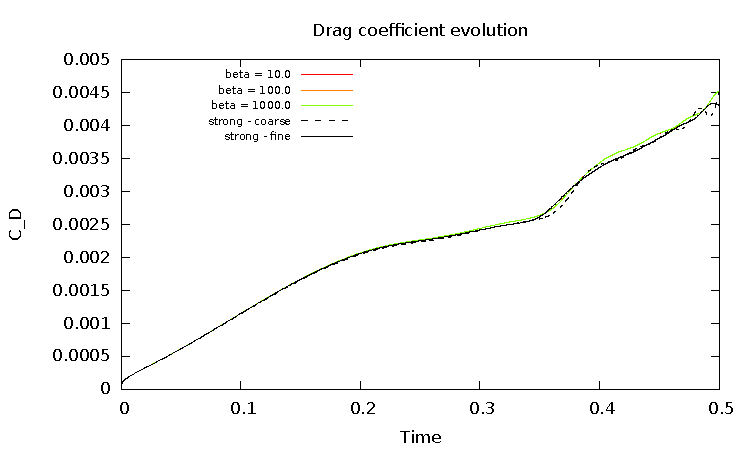
\includegraphics[width=0.6\textwidth]{Figures/Chapter8/weak/drag}}\\
  \subfigure[Lift coefficient.]{\label{fig-NACA_b_lift}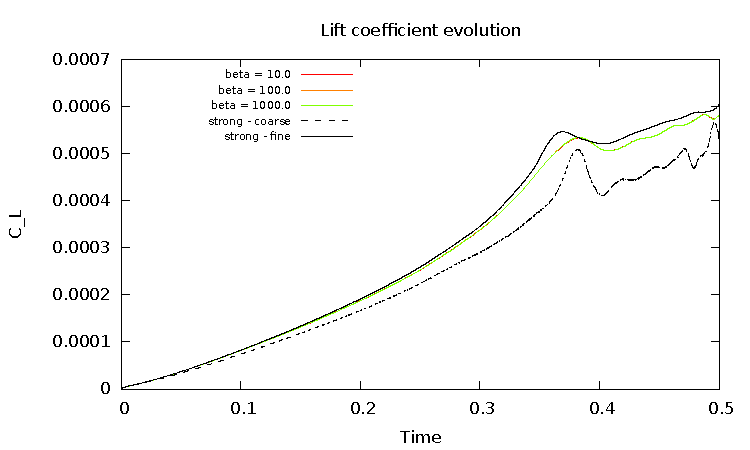
\includegraphics[width=0.6\textwidth]{Figures/Chapter8/weak/lift}}
  \caption{Drag and Lift coefficients for the 2D computation for different $ \beta $ values.}
  \label{fig-NACA_b_drag_lift}
\end{figure}
As have been shown in Section \ref{subsubsec-C7_TCF_wall_normal}, lower values of $ \beta $ result in lower computational time, so we will favour $ \beta=10 $ for the following computations.

\subsection{Strong vs weak BCs}
In order to see the difference on the computed solution when using strong or weak Dirichlet boundary conditions, we show the mean flow for both, fine and coarse meshes, respectively, averaging the results obtained between $ t=0.8 $ and $ t=1.0 $.

In \Fig{NACA_mean_velo} we depict the mean velocity magnitude for the case in which we impose strongly the boundary conditions in a fine mesh (\Fig{NACA_mean_velo_fine}) and the case in which we impose weakly the boundary conditions in a coarse mesh (\Fig{NACA_mean_velo_coarse}). We see the same velocity distribution in both cases, with very tiny changes between them. In order to better see the difference between both solutions, in \Fig{NACA_mean_velo_diff} we depict the mean velocity isolines for the two cases. We see that the solution is very similar for the two computations, conserving the same structures 
\begin{figure}[h!]
  \centering
  \subfigure[Fine mesh, strong BCs.]{\label{fig-NACA_mean_velo_fine}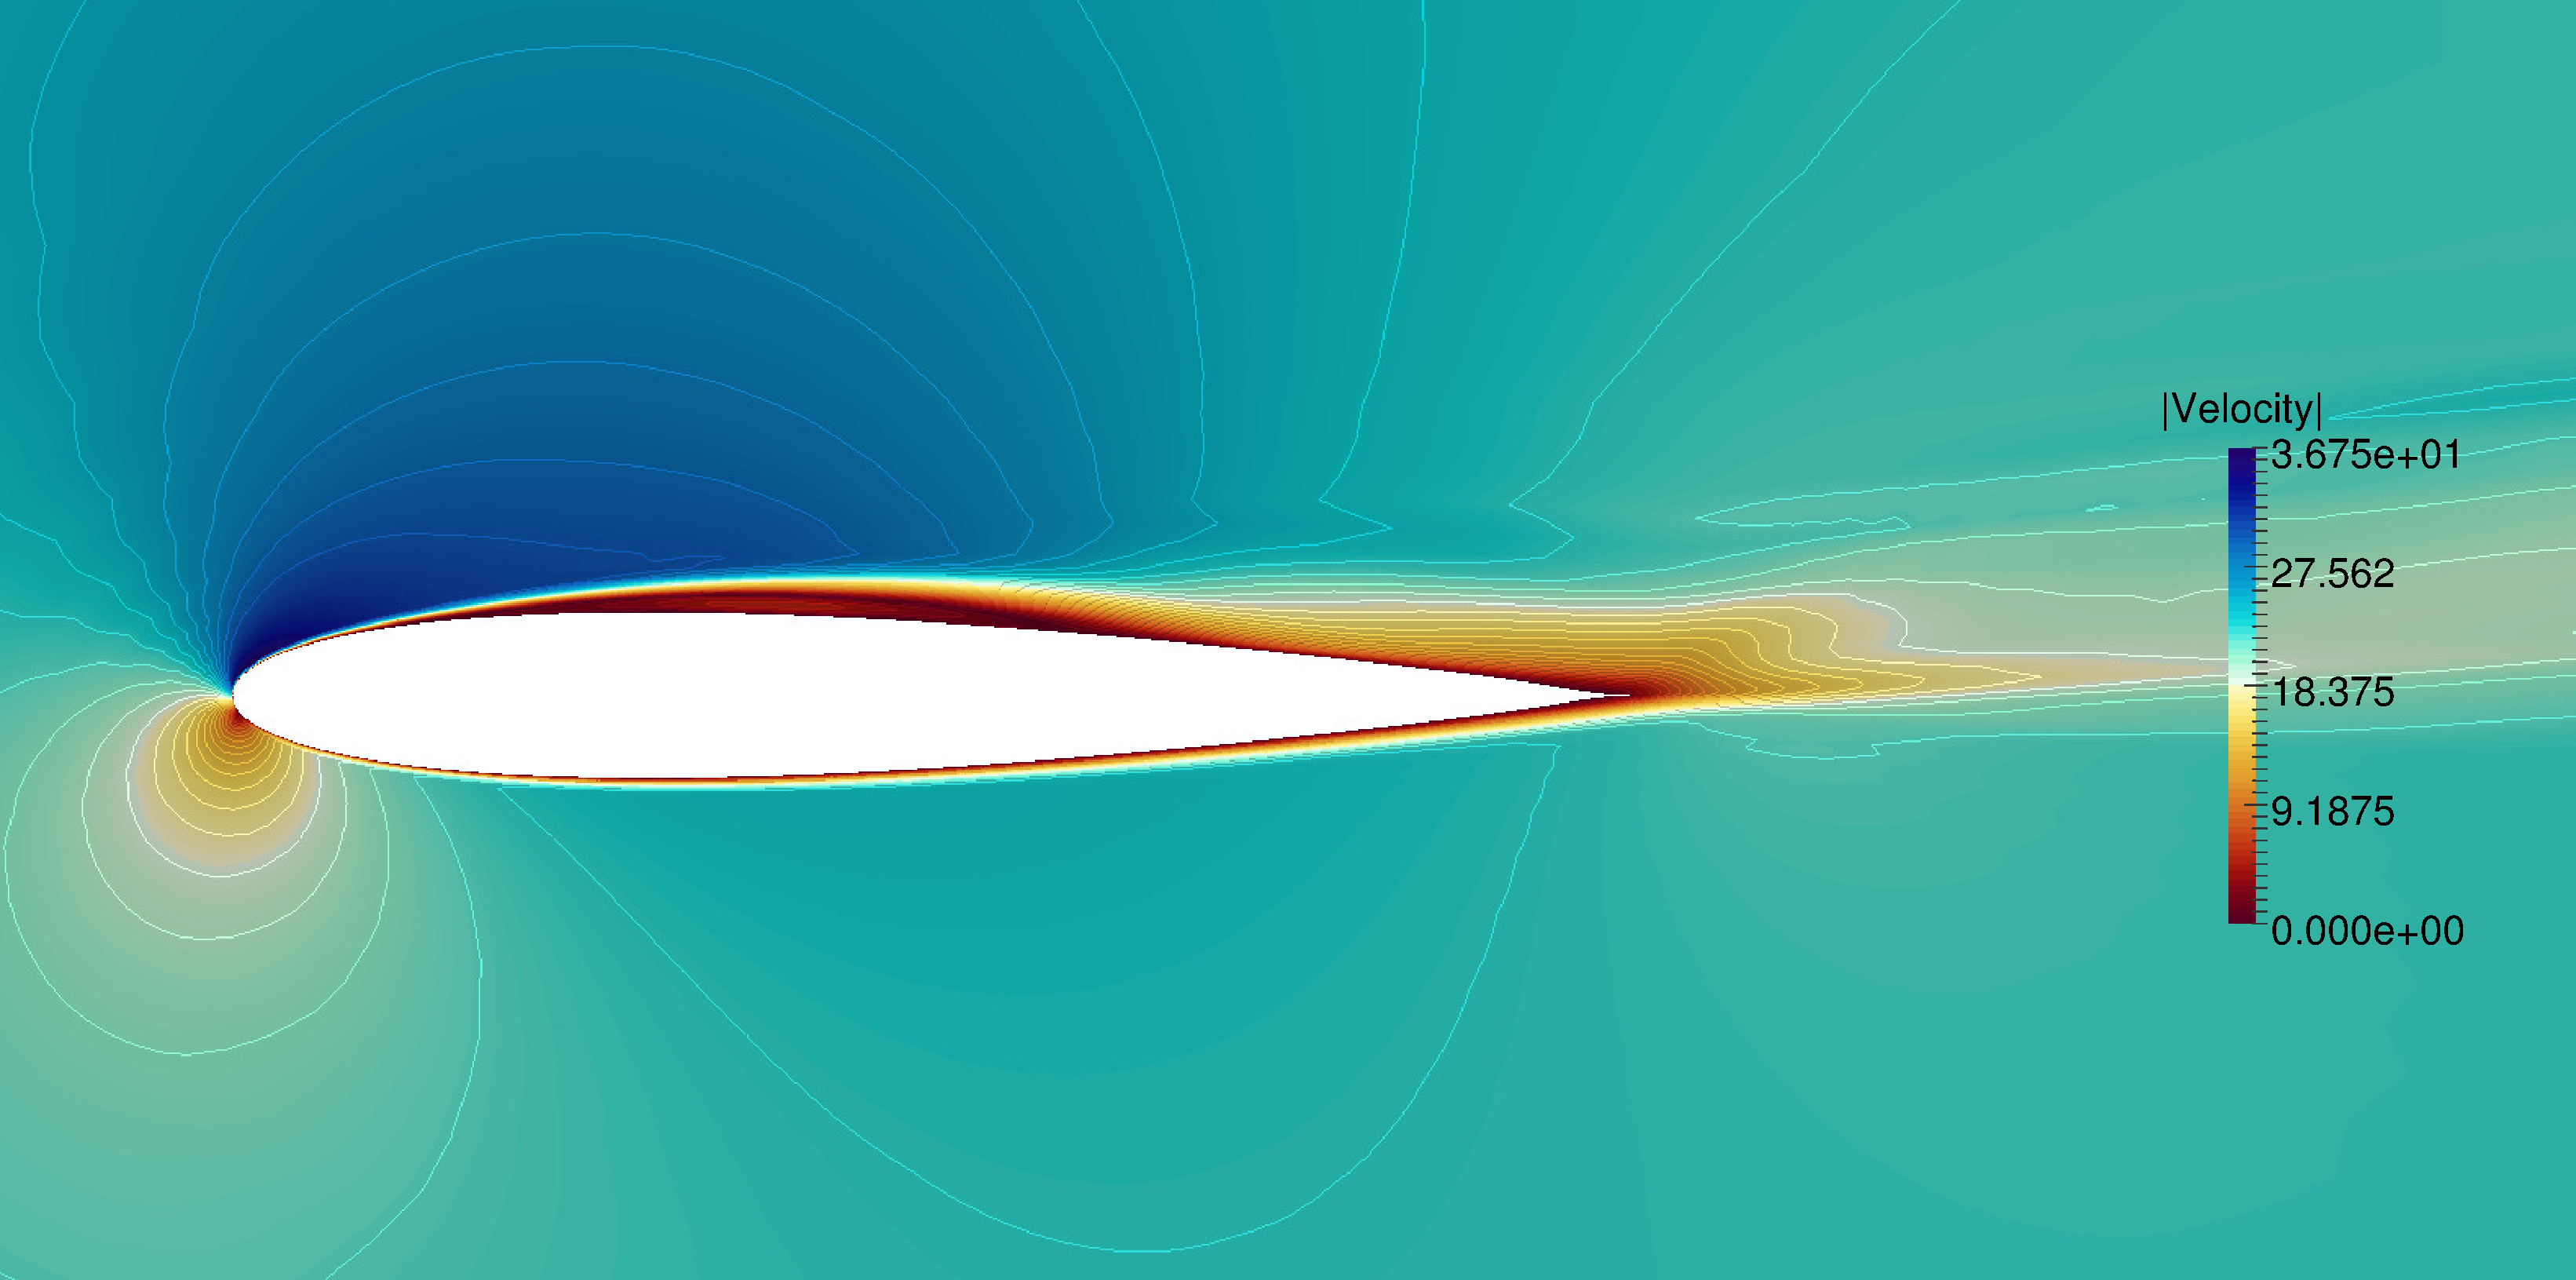
\includegraphics[width=0.7\textwidth]{Figures/Chapter8/strong/velo_mean_fine}}\\
  \subfigure[Coarse mesh, weak BCs.]{\label{fig-NACA_mean_velo_coarse}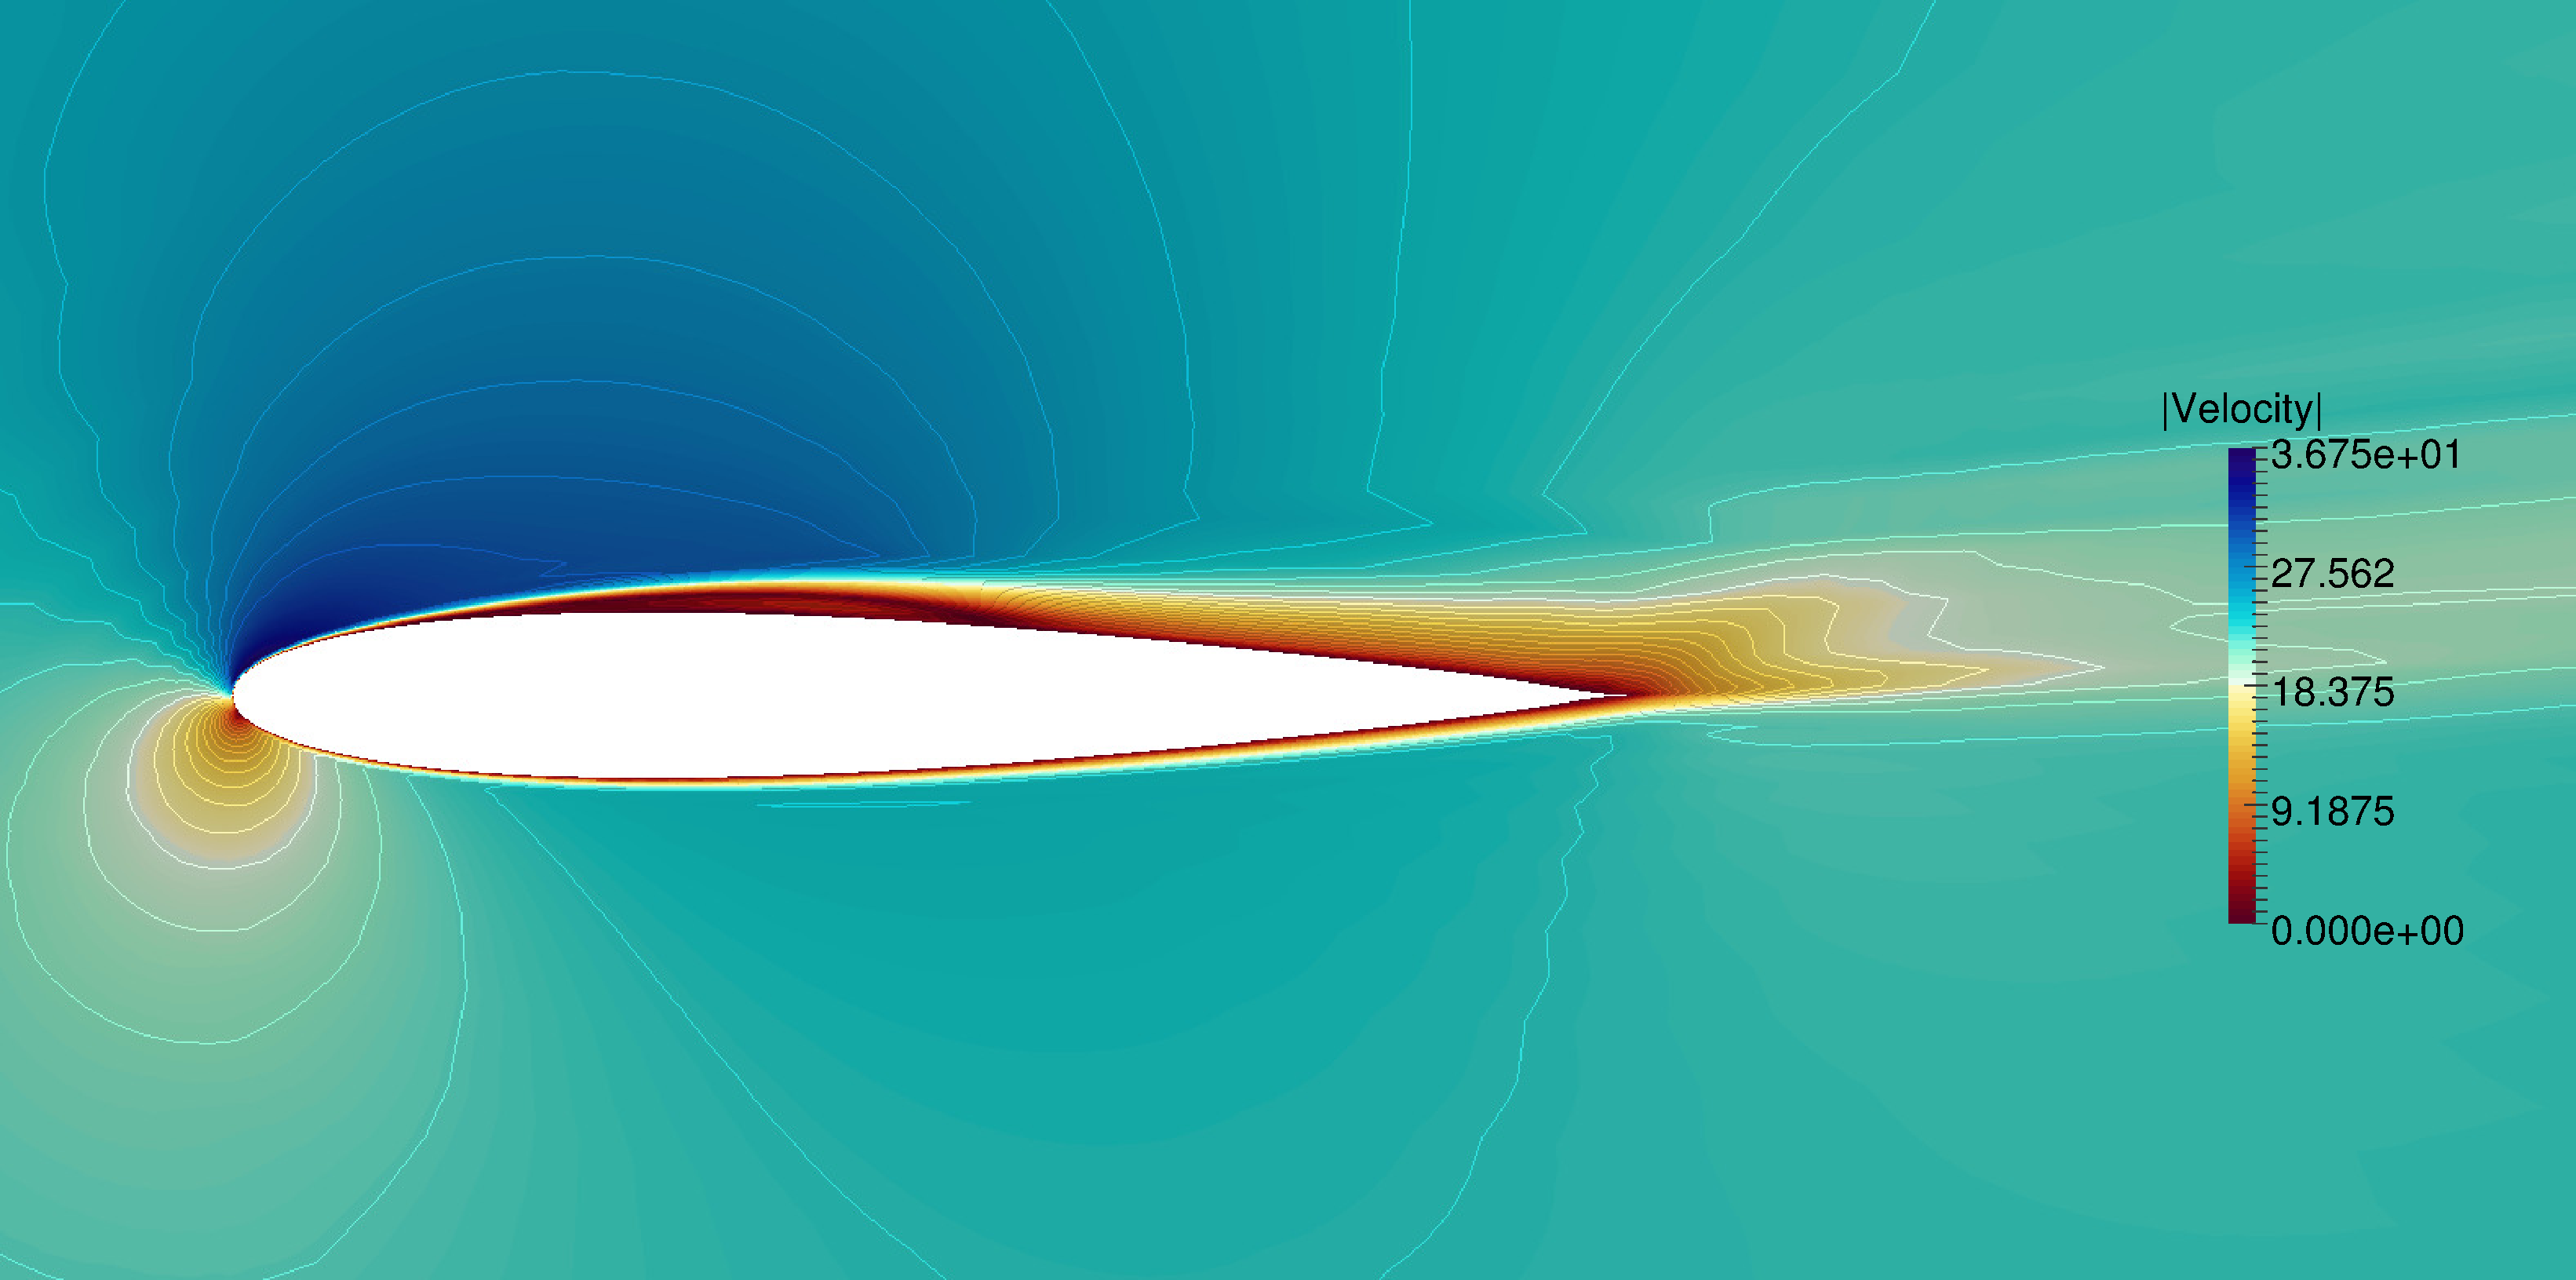
\includegraphics[width=0.7\textwidth]{Figures/Chapter8/strong/velo_mean_coarse}}\\
  \subfigure[Velocity magnitude isolines.]{\label{fig-NACA_mean_velo_diff}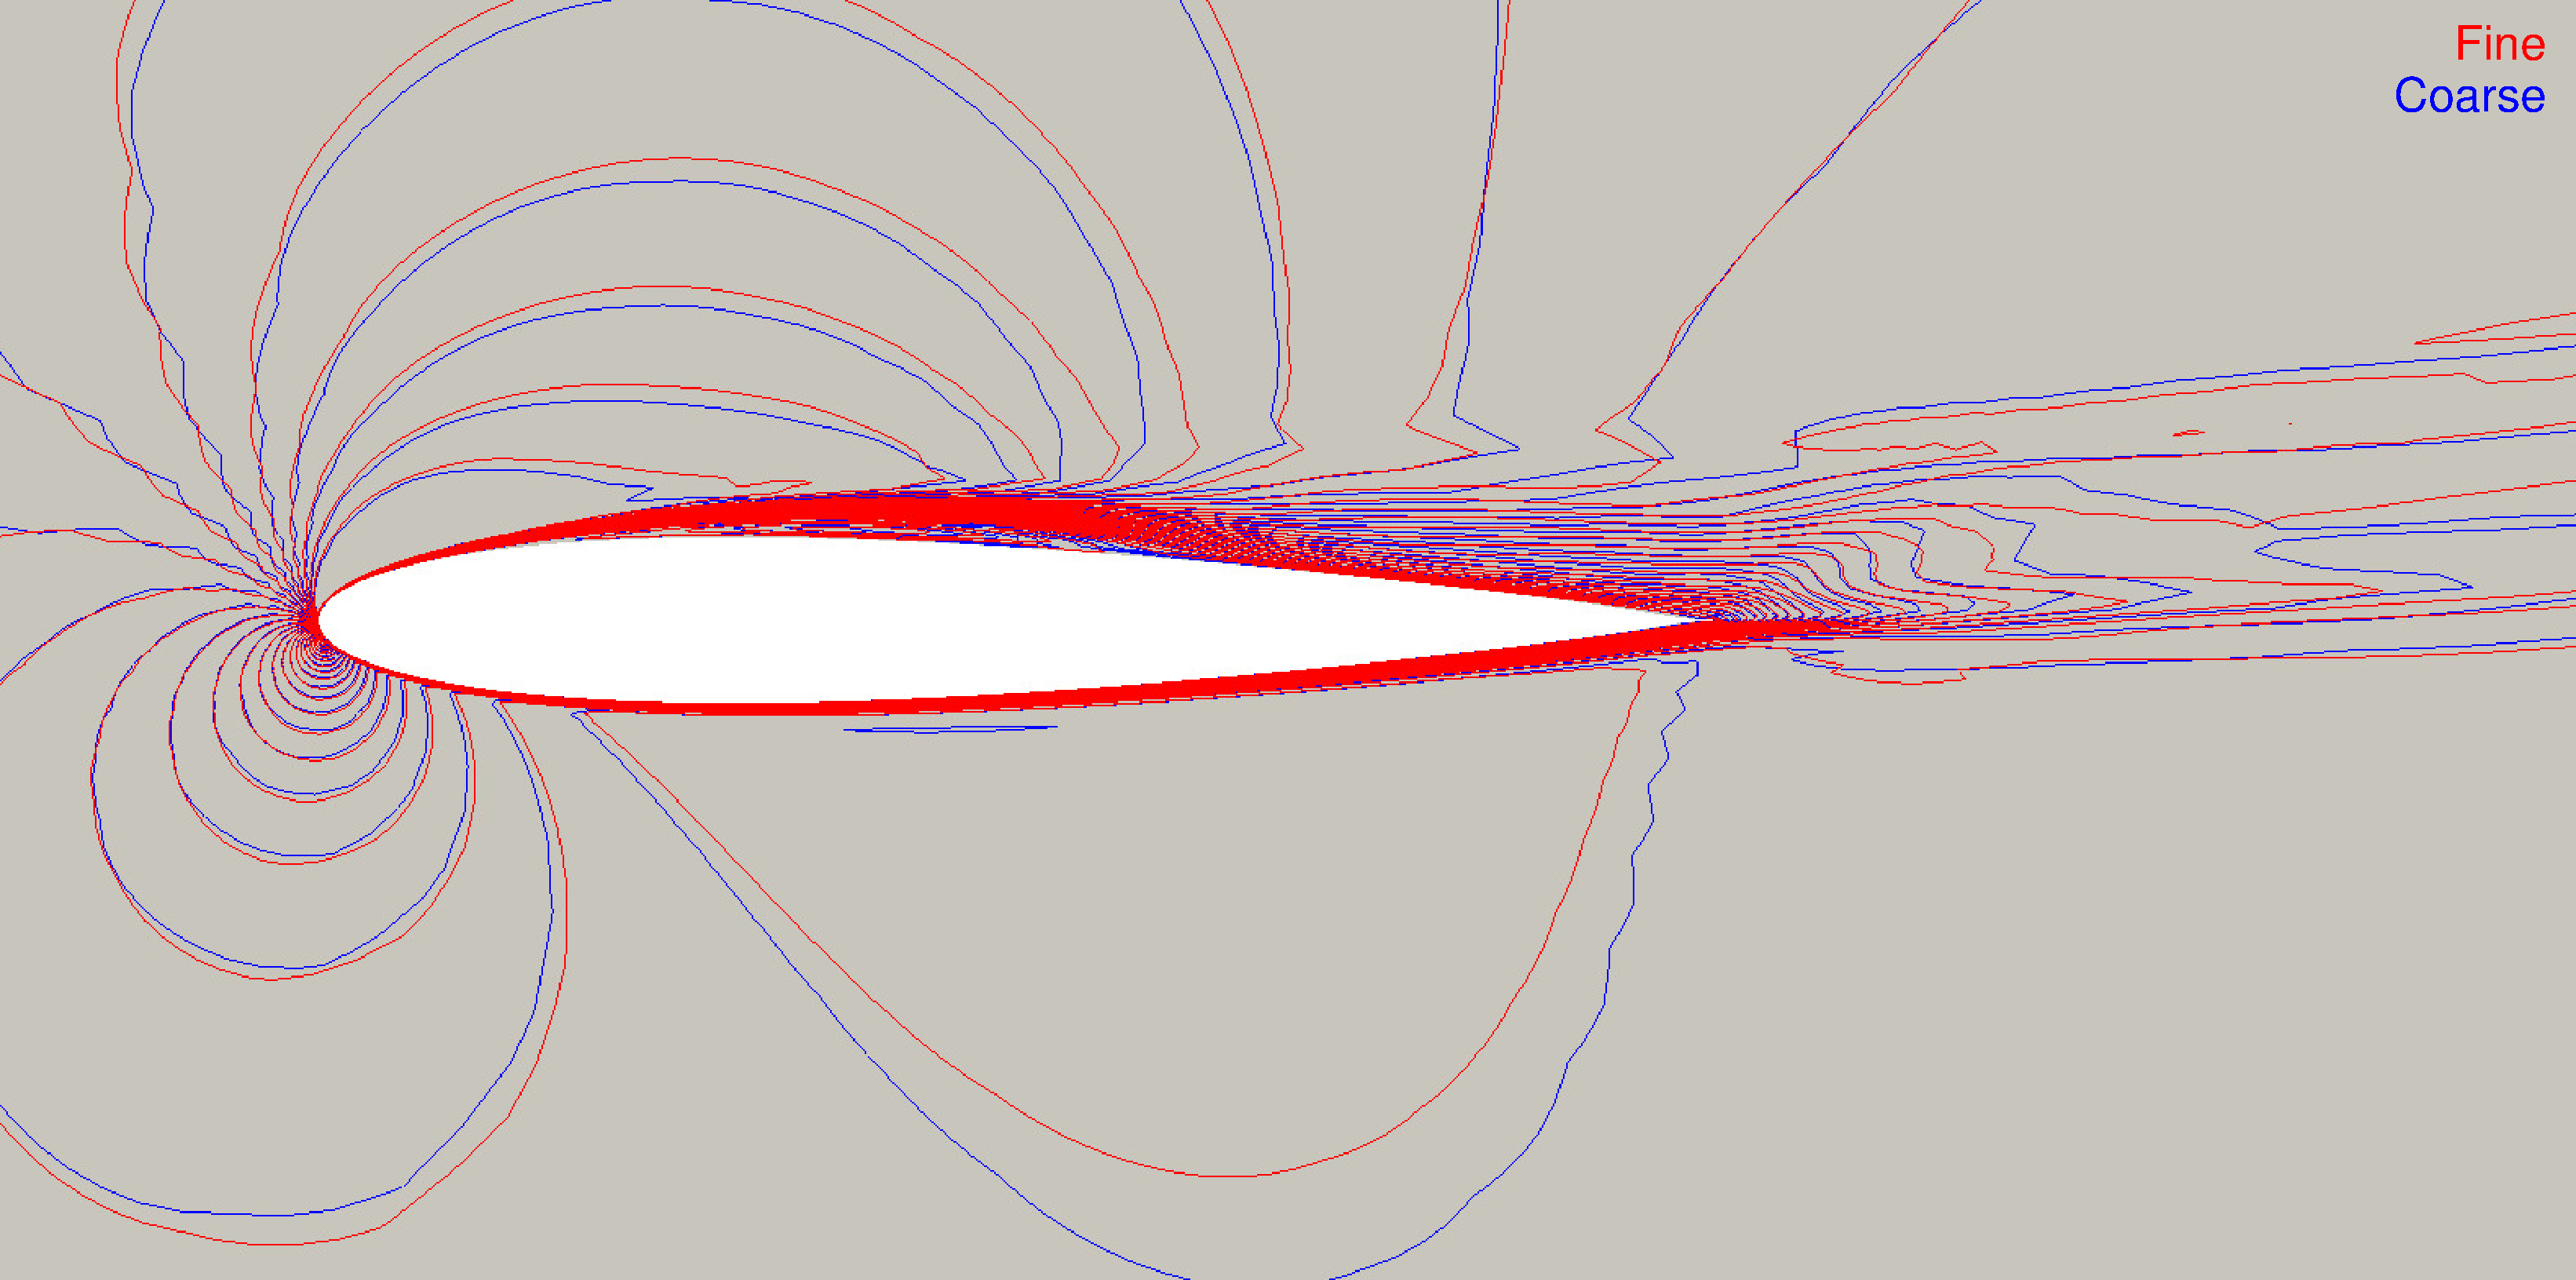
\includegraphics[width=0.7\textwidth]{Figures/Chapter8/strong/diff_velo_mean}}
  \caption{Mean velocity magnitude for the fine and coarse meshes.}
  \label{fig-NACA_mean_velo}
\end{figure}
Focusing on the velocity fluctuations, in \Fig{NACA_dev_velo} we depict the standard deviation of the velocity magnitude computed from $ t=0.8 $ to $ t=1.0 $. In this case, we also see very litle differences, noting that the fluctuating regions are located at the same positions in both cases.
\begin{figure}[h!]
  \centering
  \subfigure[Fine mesh, strong BCs.]{\label{fig-NACA_dev_velo_fine}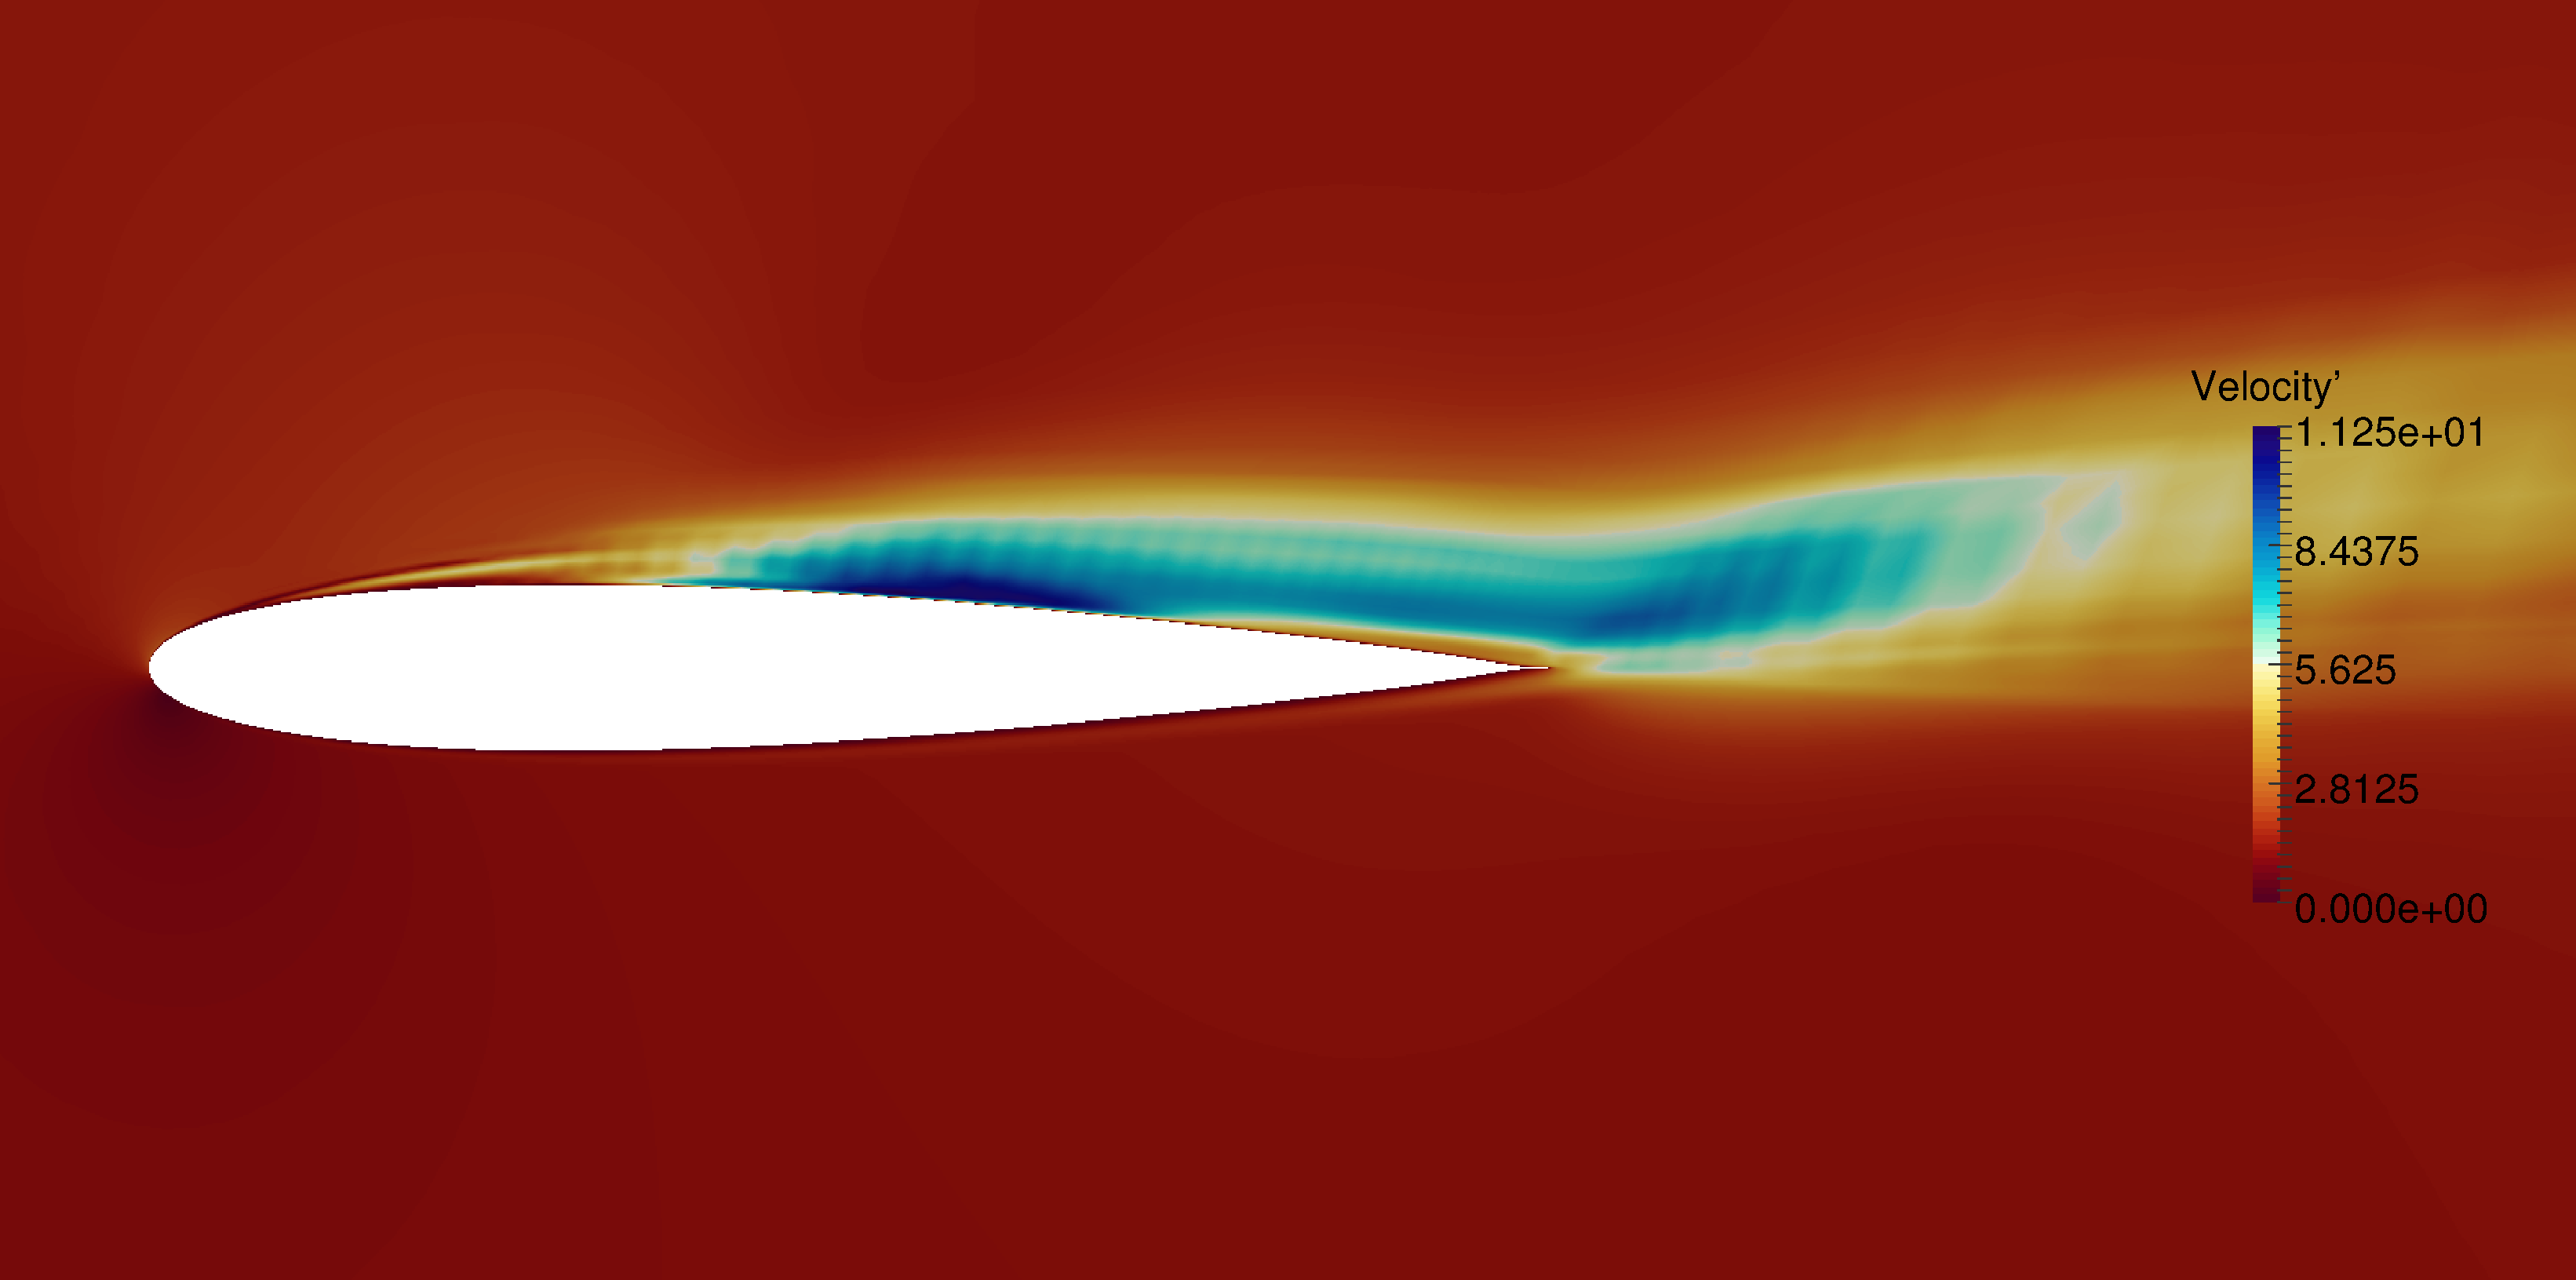
\includegraphics[width=0.49\textwidth]{Figures/Chapter8/strong/velo_dev_fine}}
  \subfigure[Coarse mesh, weak BCs.]{\label{fig-NACA_dev_velo_coarse}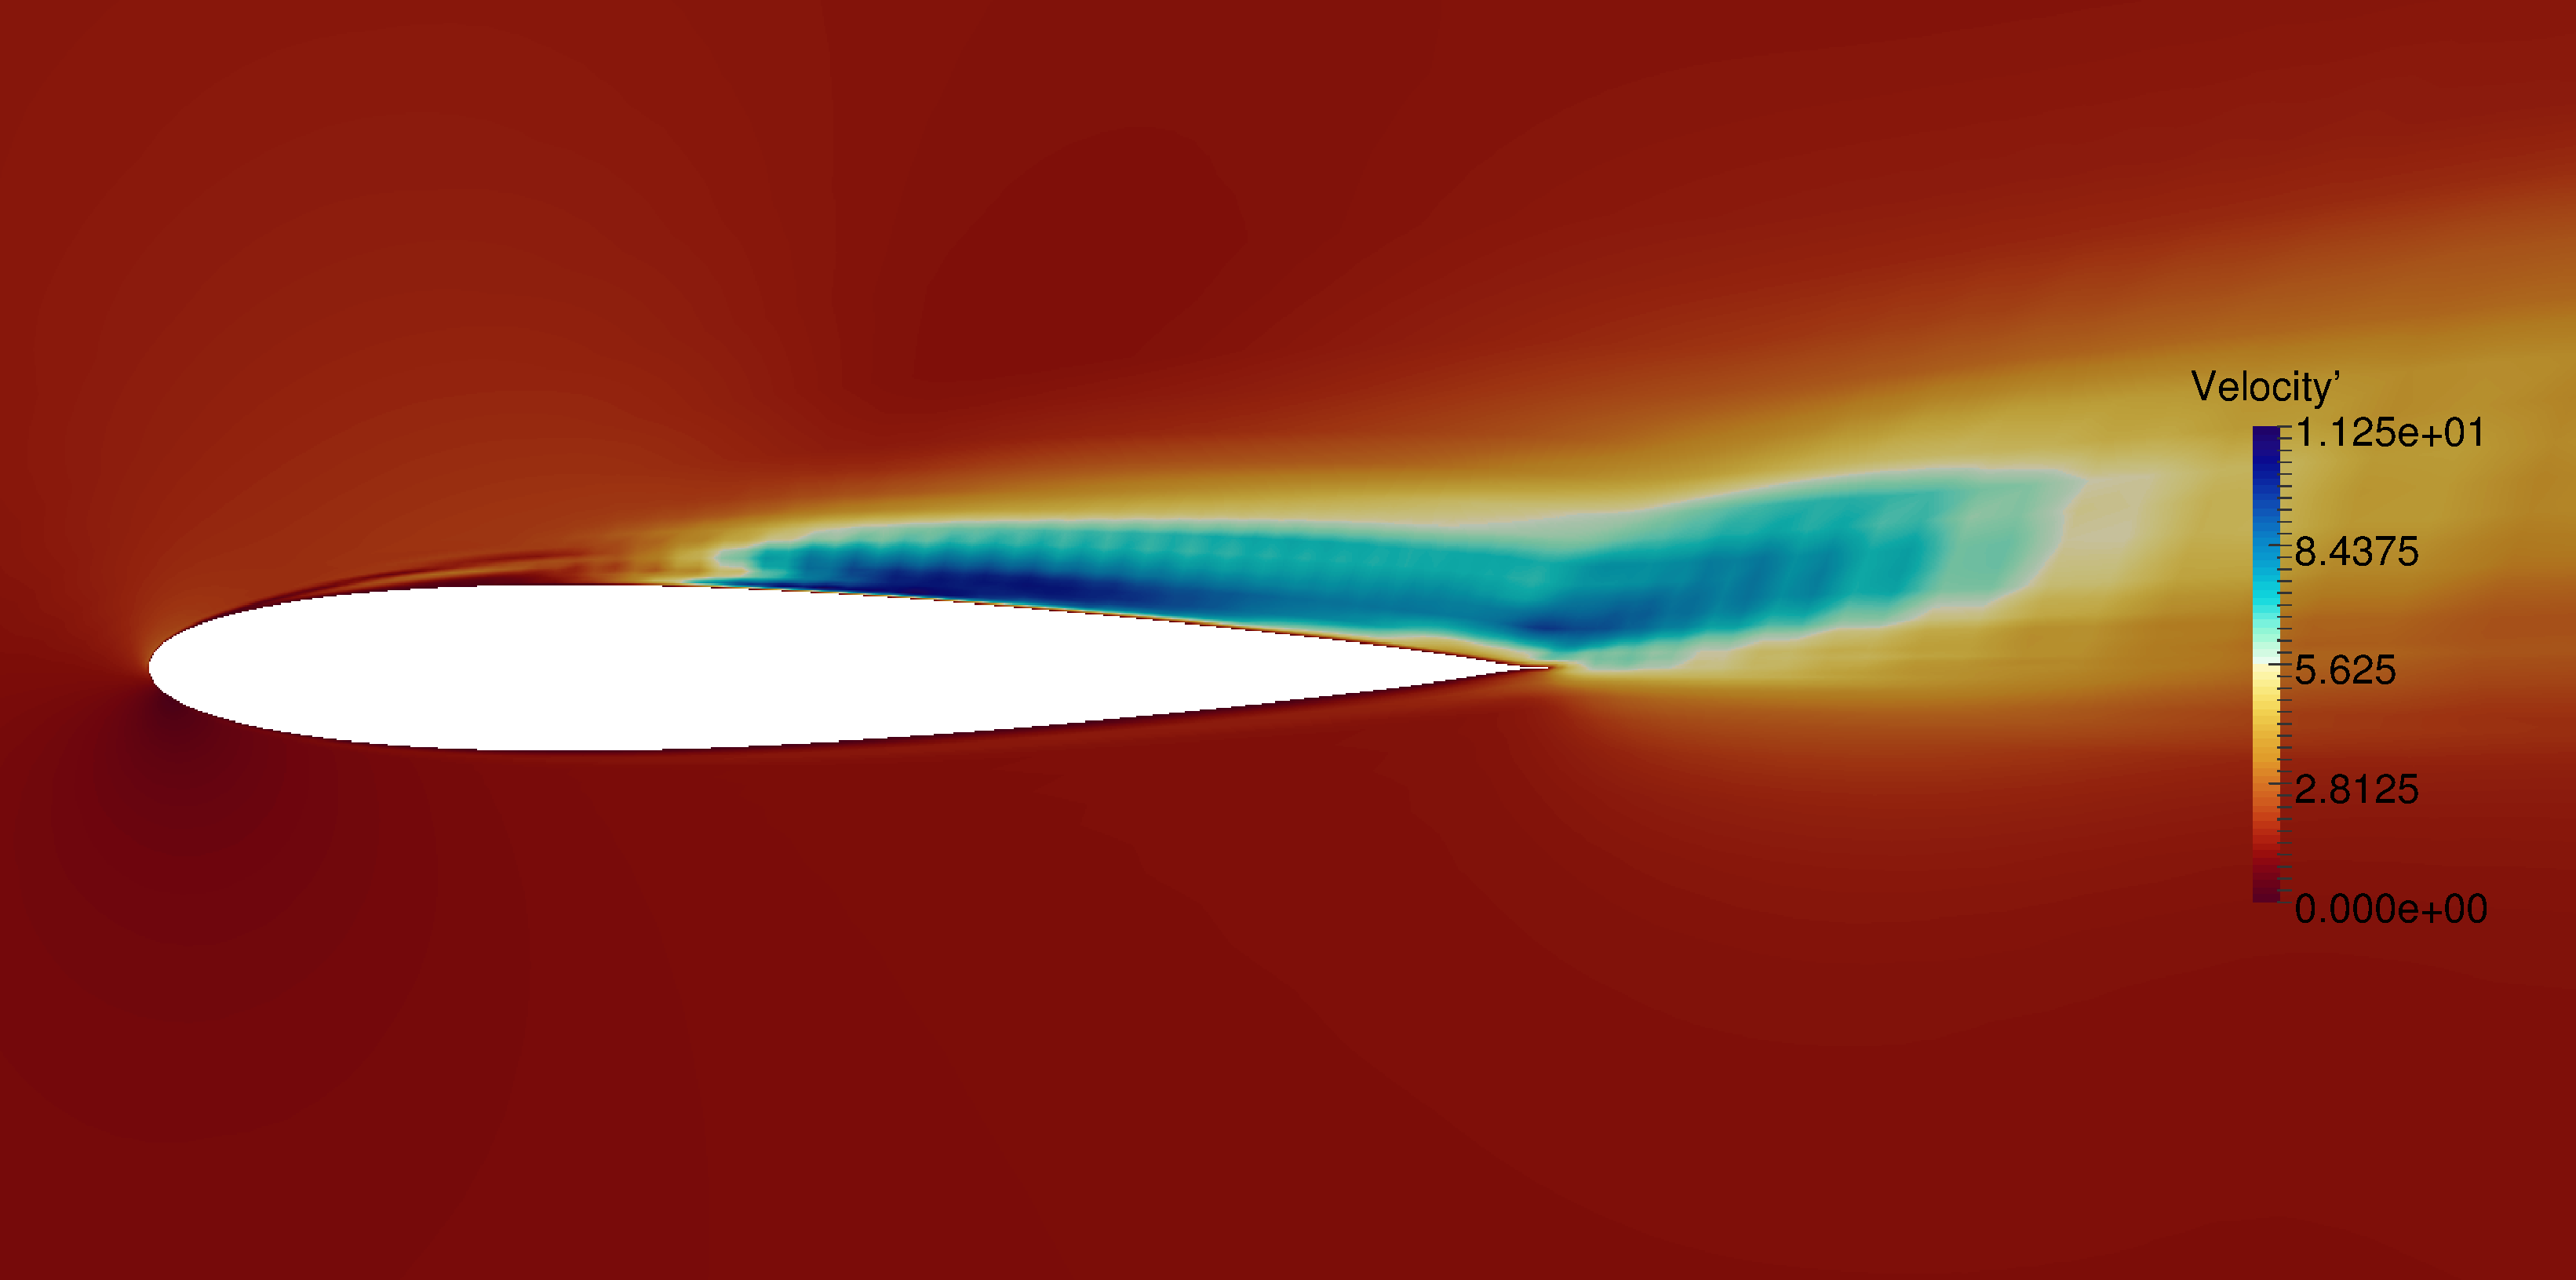
\includegraphics[width=0.49\textwidth]{Figures/Chapter8/strong/velo_dev_coarse}}
  \caption{Standard deviation of the velocity magnitude for the fine and coarse meshes.}
  \label{fig-NACA_dev_velo}
\end{figure}

Looking now at the mean pressure plots depicted in \Fig{NACA_mean_press} we can observe the same similarities between the two computations. In \Fig{NACA_mean_press_fine} the fine mesh with strong BCs solution is ploted, while the solution in the coarse mesh and weak BCs is shown in \Fig{NACA_mean_press_coarse}. The little differences between the two results can be distinguished in \Fig{NACA_mean_press_diff}, where the pressure isolines are depicted.
\begin{figure}[h!]
  \centering
  \subfigure[Fine mesh, strong BCs.]{\label{fig-NACA_mean_press_fine}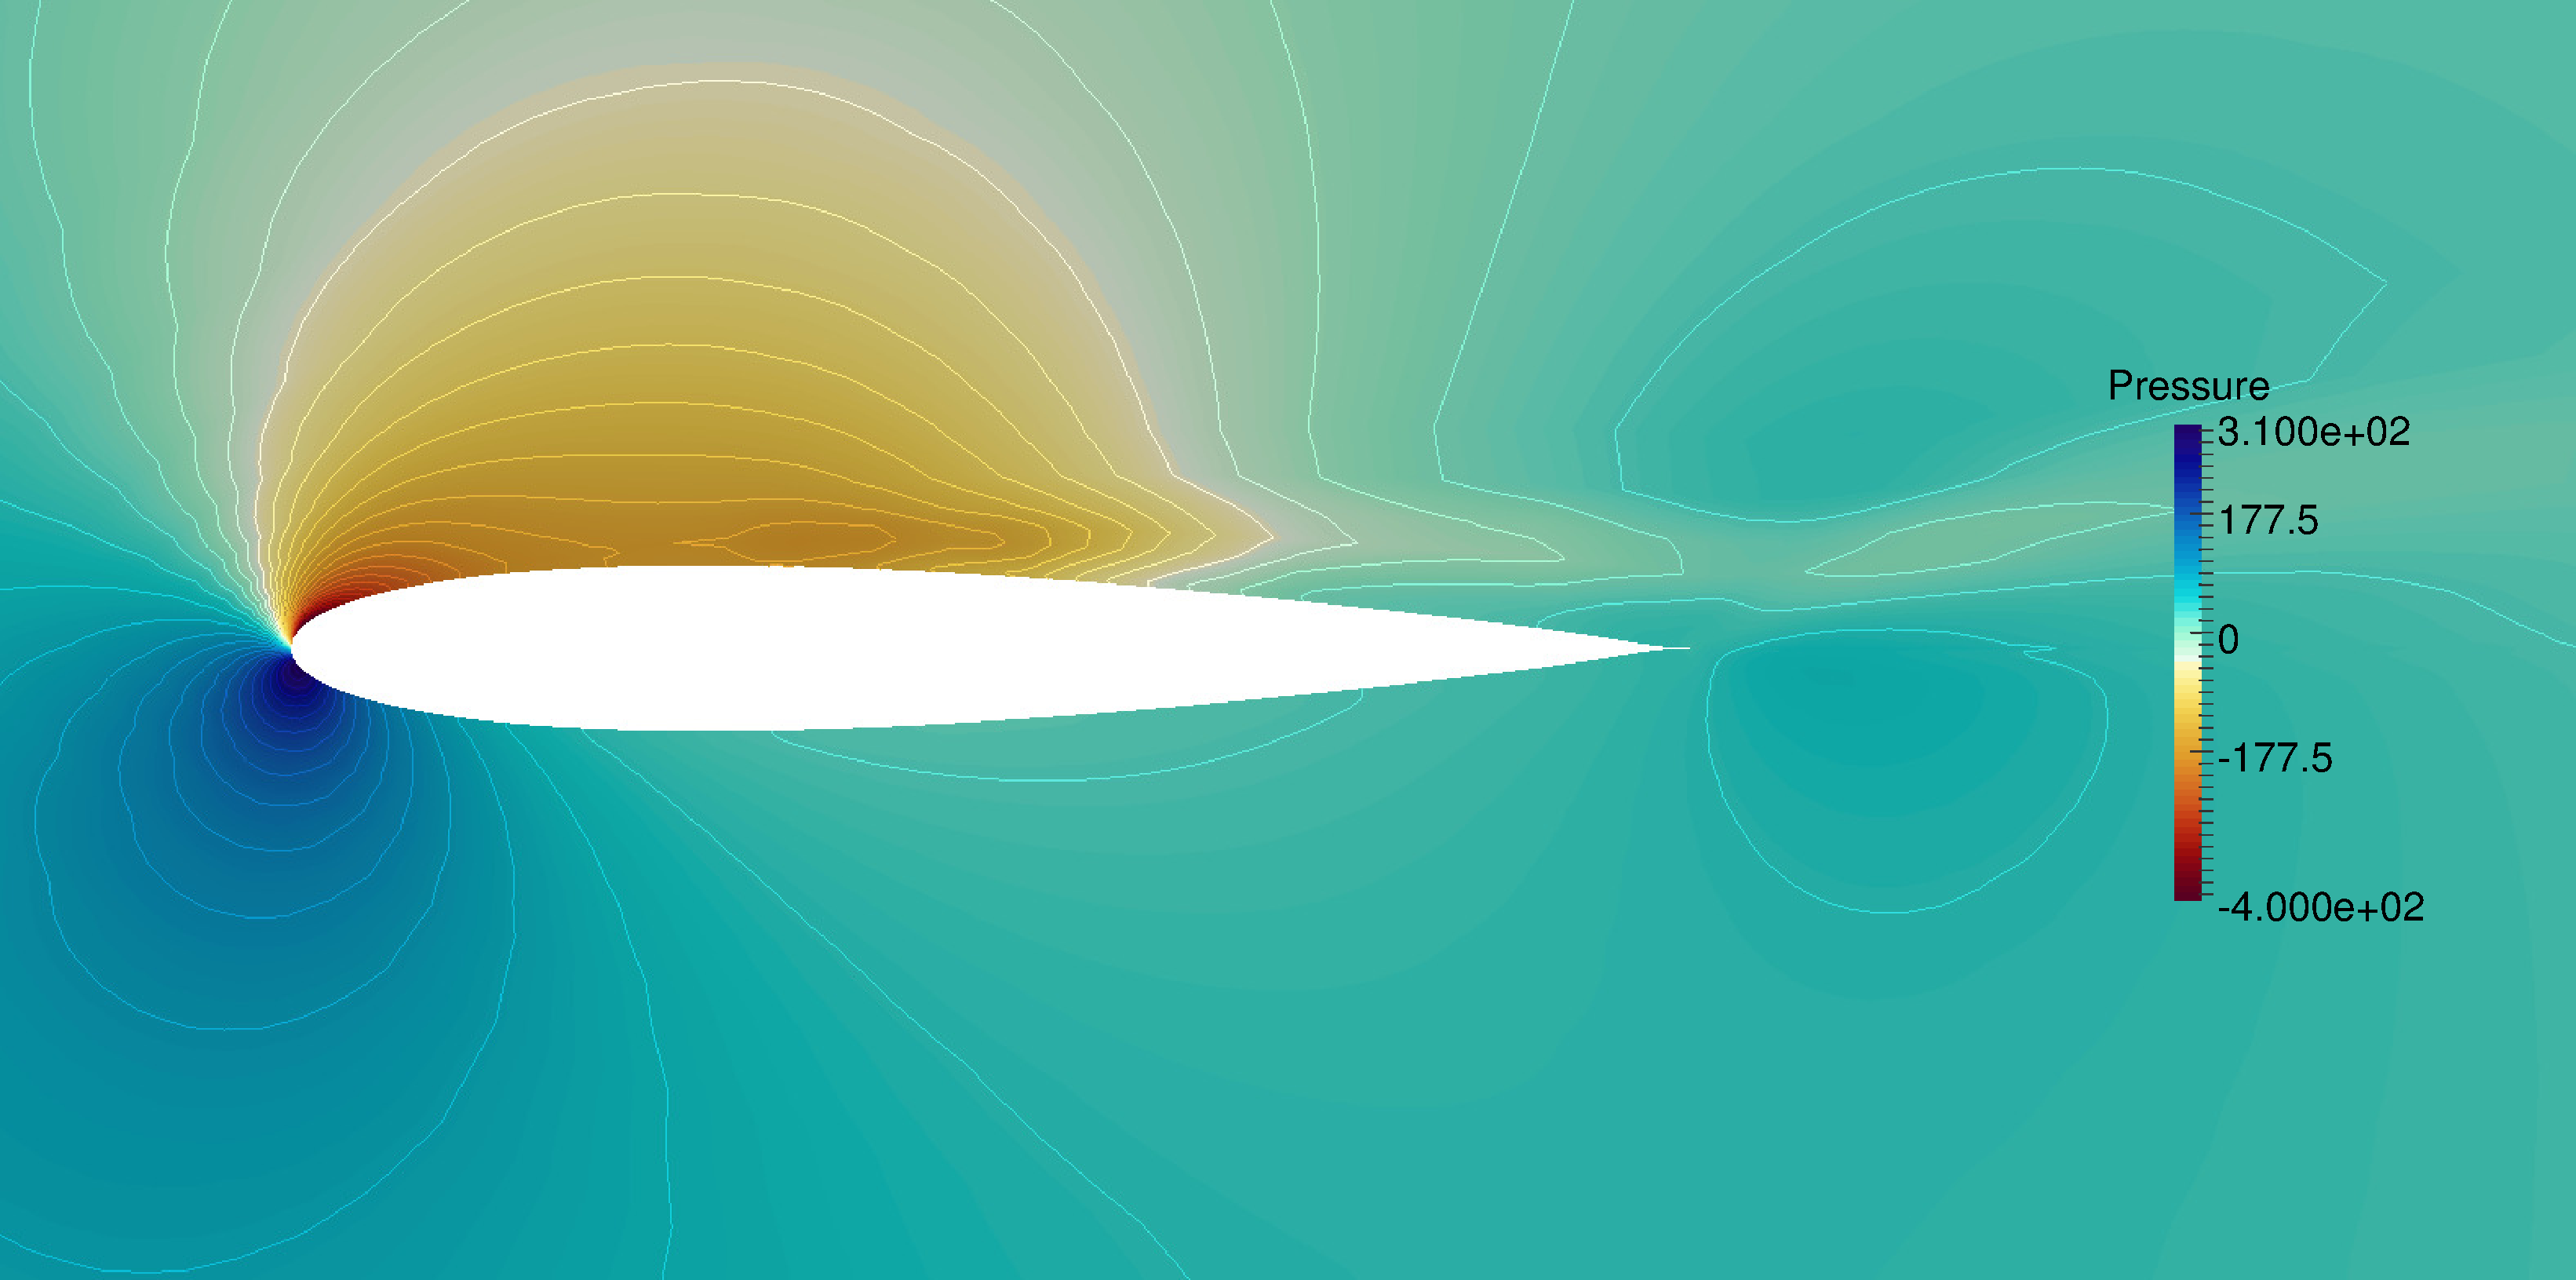
\includegraphics[width=0.7\textwidth]{Figures/Chapter8/strong/press_mean_fine}}\\
  \subfigure[Coarse mesh, weak BCs.]{\label{fig-NACA_mean_press_coarse}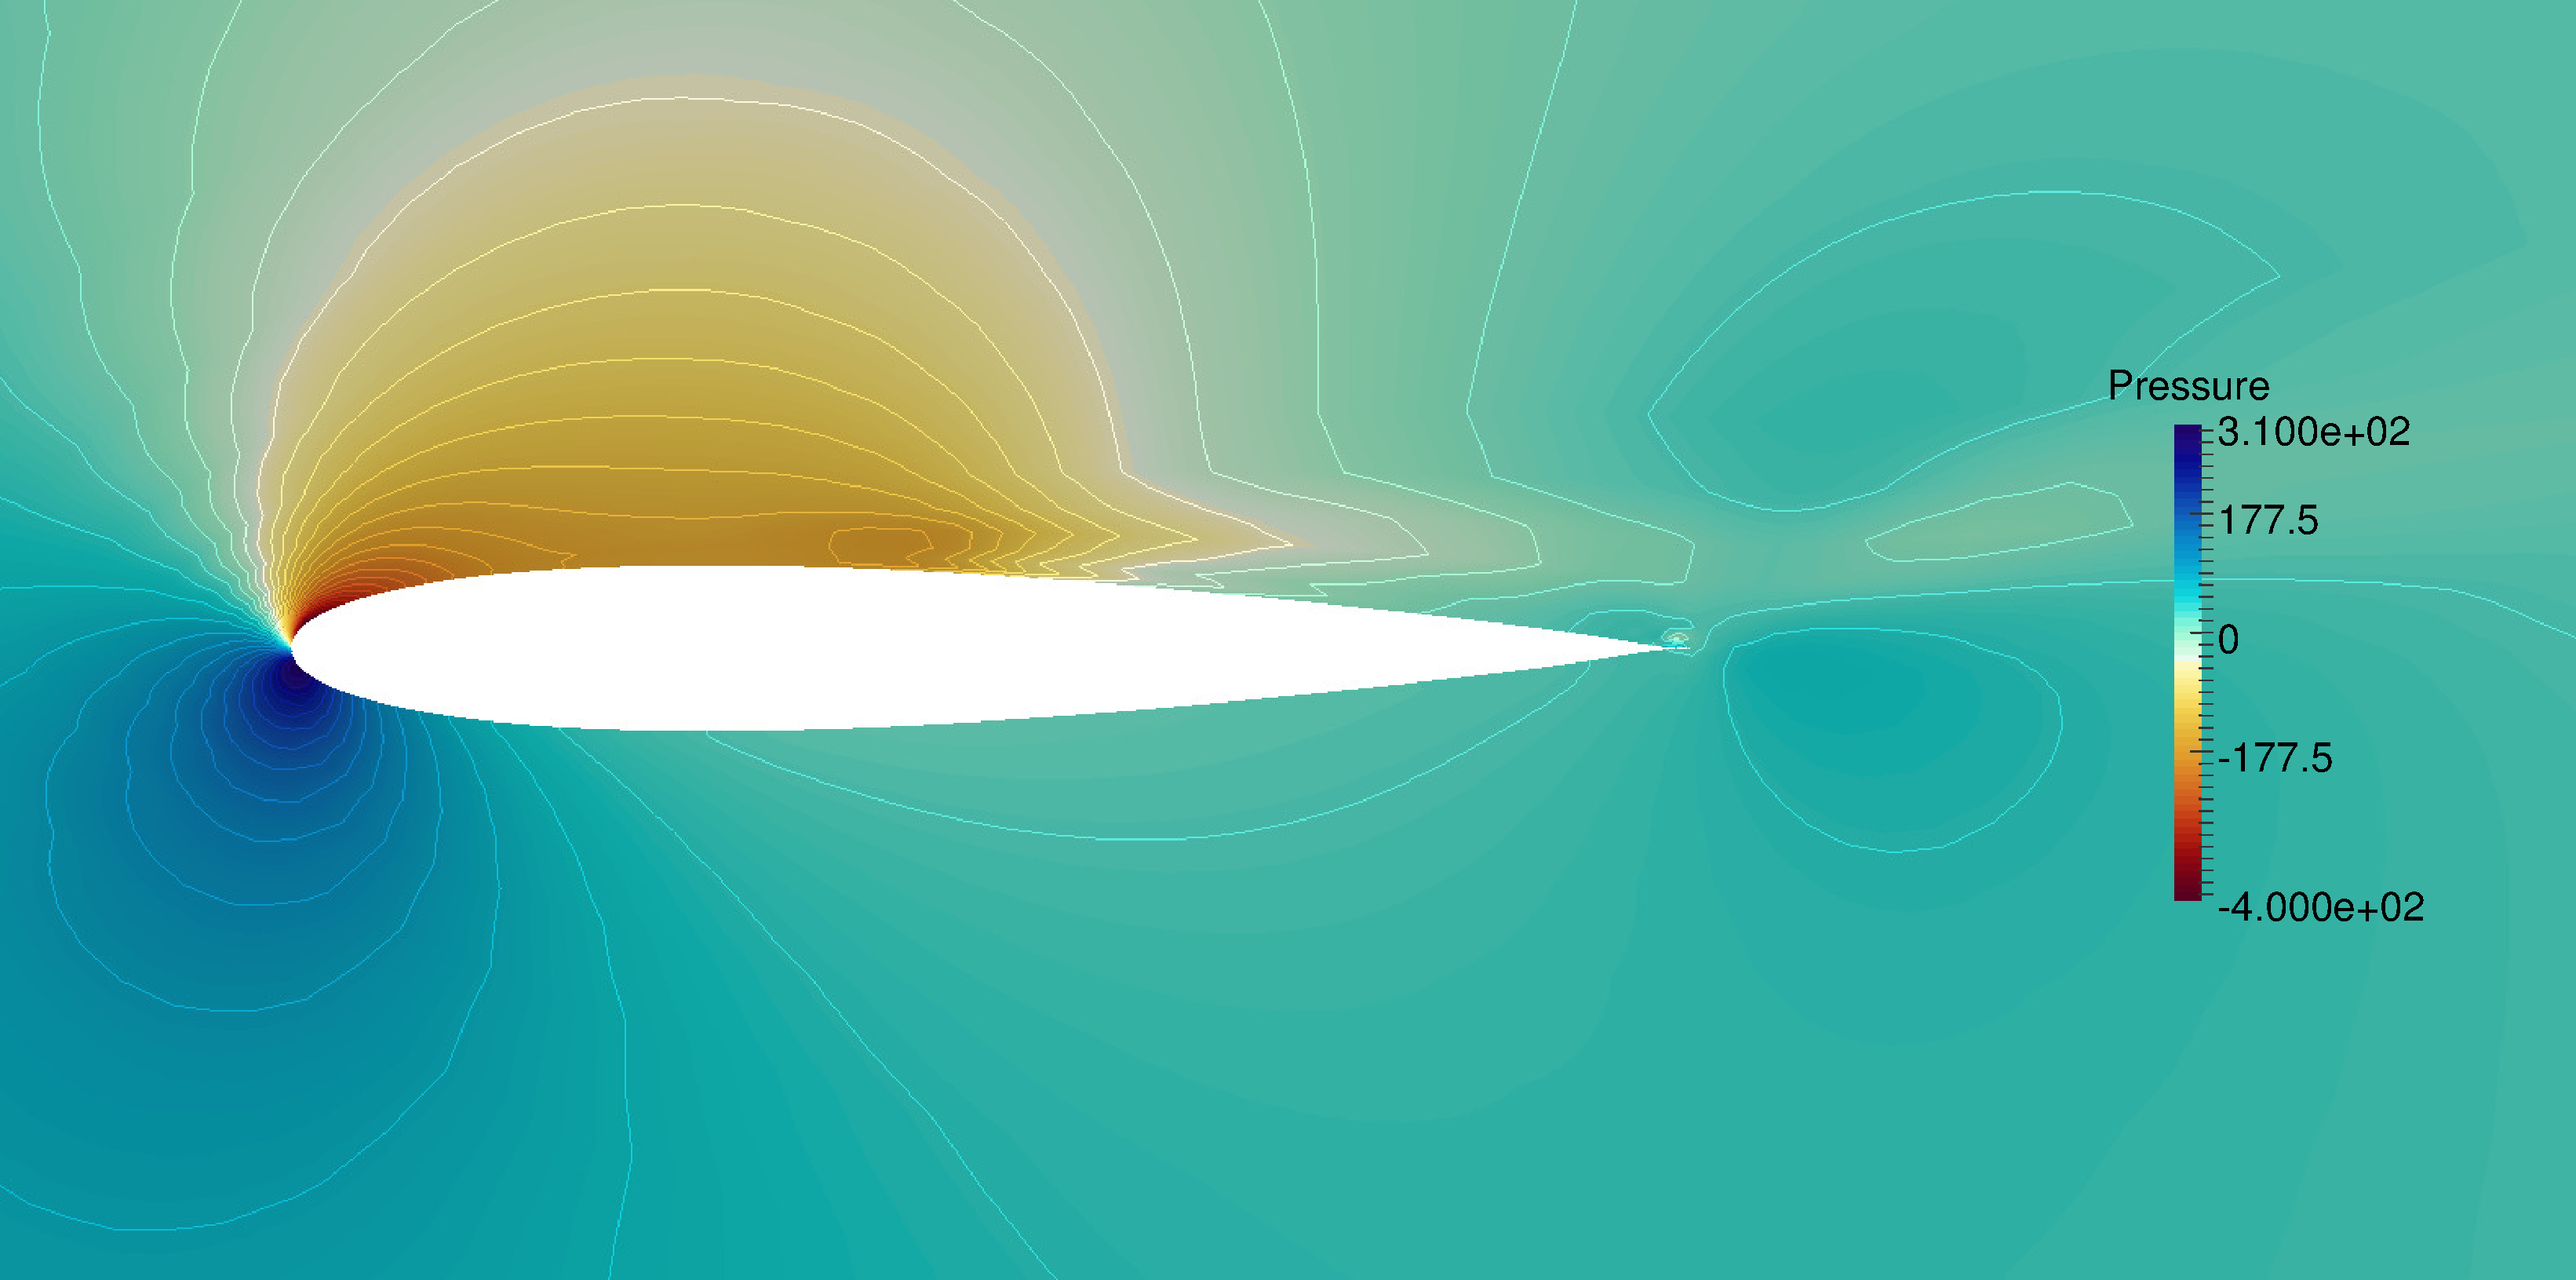
\includegraphics[width=0.7\textwidth]{Figures/Chapter8/strong/press_mean_coarse}}\\
  \subfigure[Velocity magnitude isolines.]{\label{fig-NACA_mean_press_diff}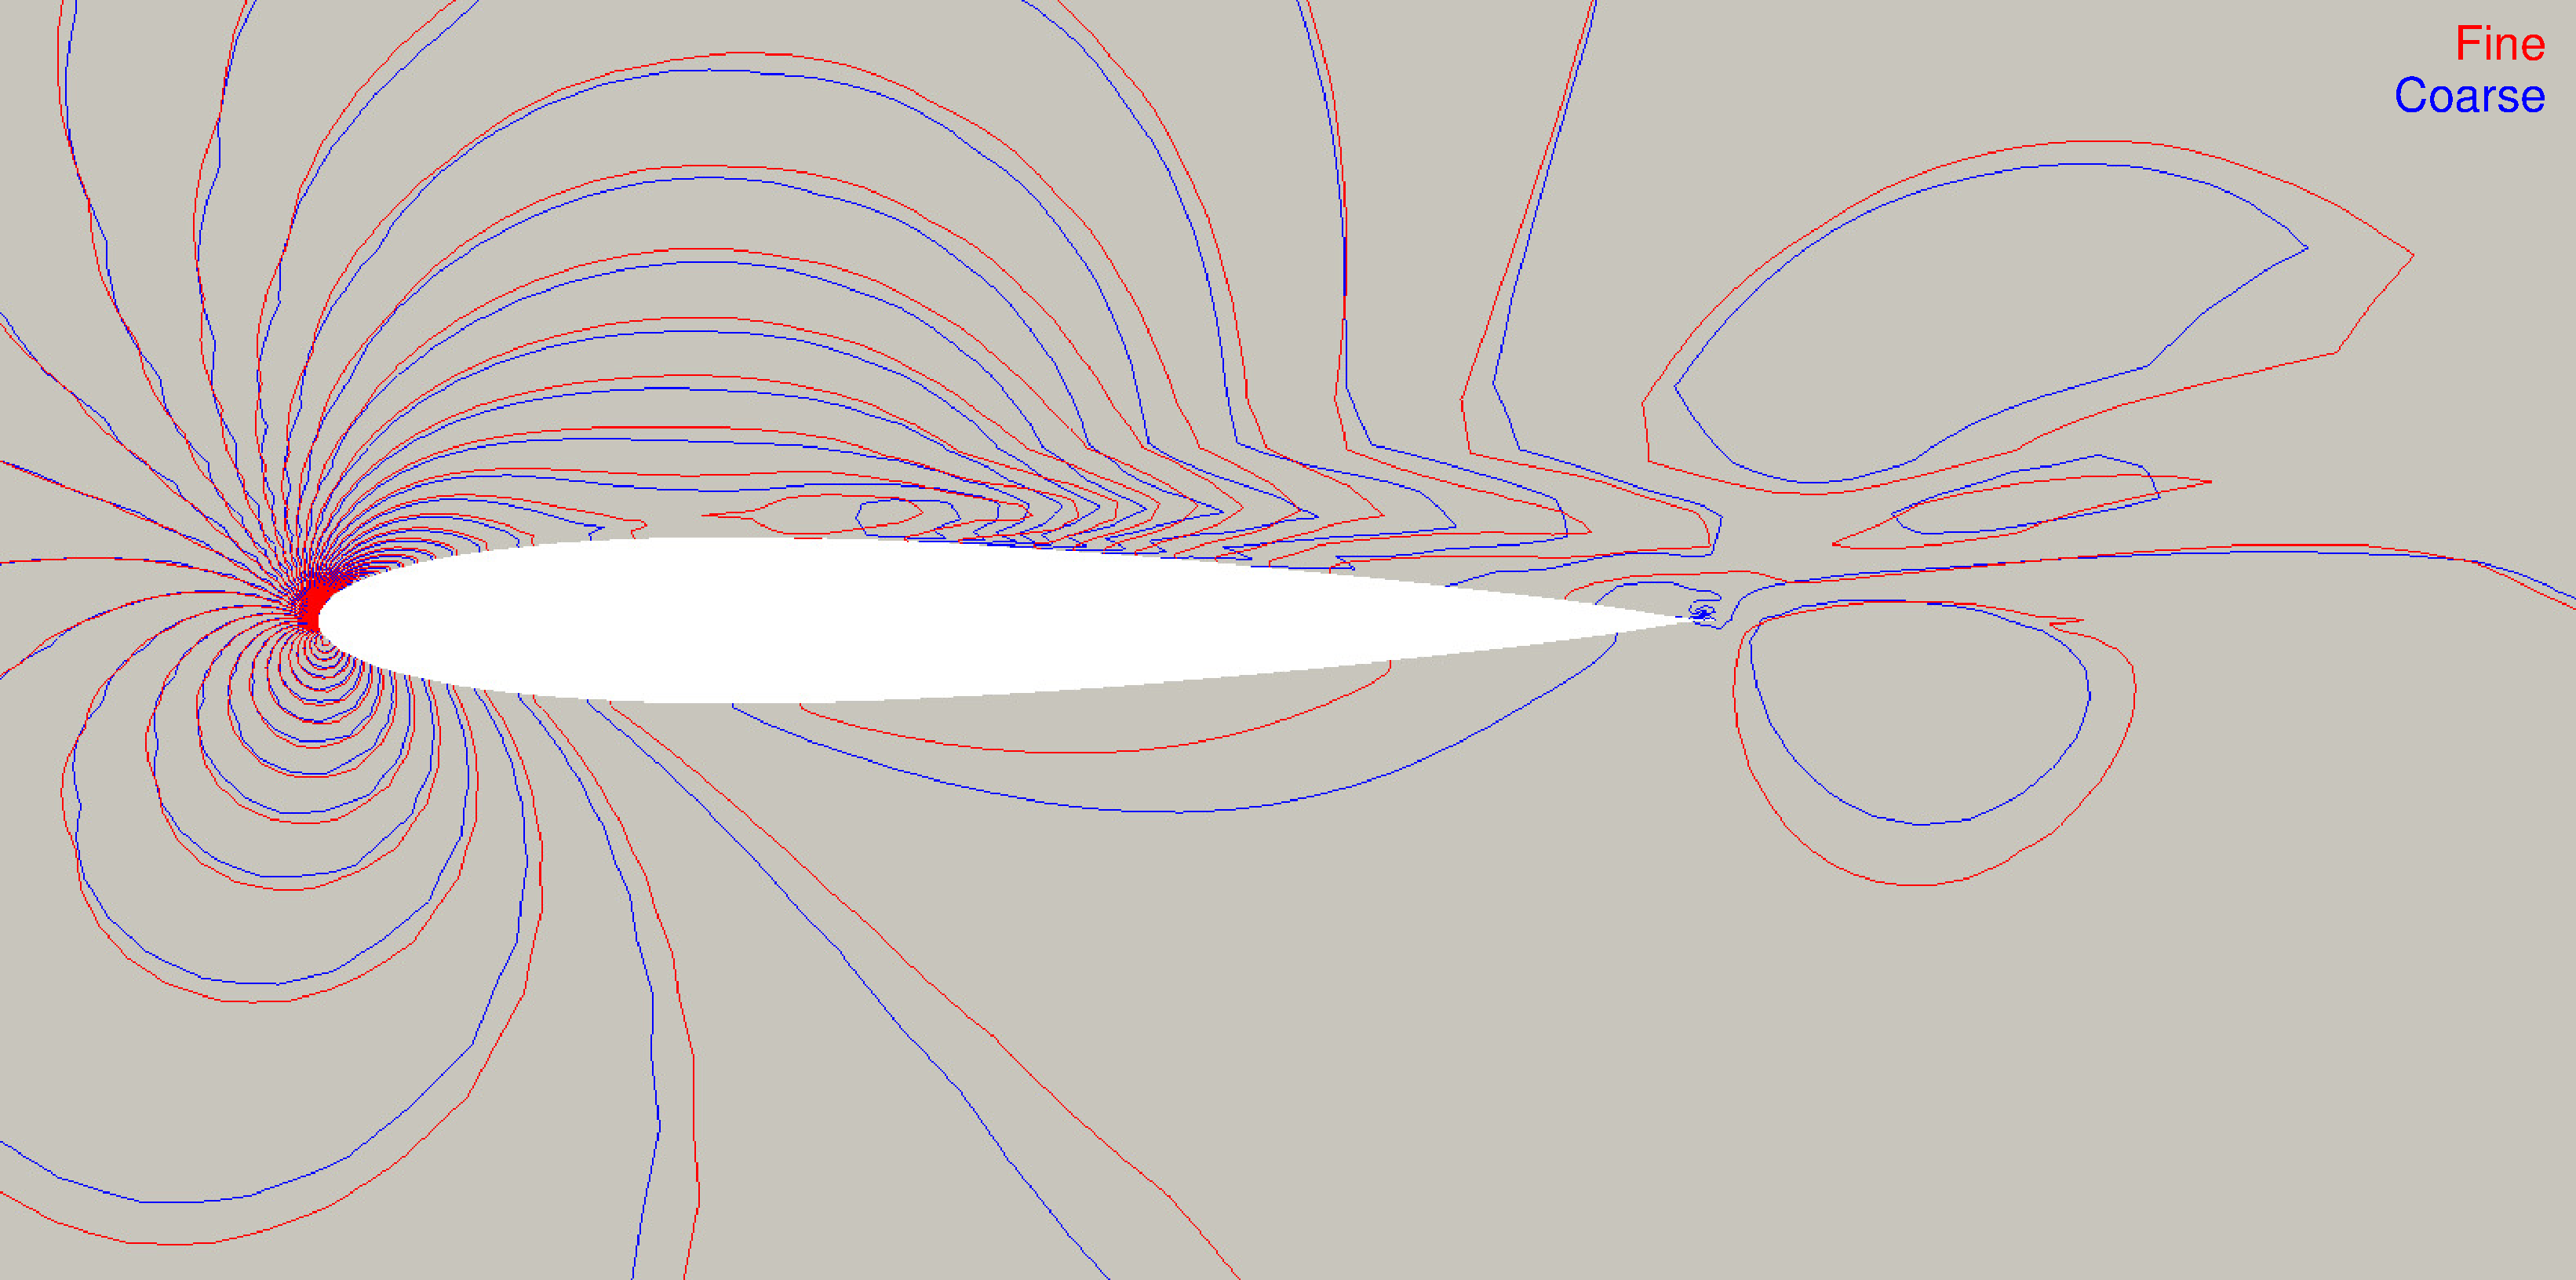
\includegraphics[width=0.7\textwidth]{Figures/Chapter8/strong/diff_press_mean}}
  \caption{Mean pressure for the fine and coarse meshes.}
  \label{fig-NACA_mean_press}
\end{figure}

\subsection{Instantaneous flowfields for the 3D case}
Once analysed the efect of using weak Dirichlet boundary conditions on a two-dimensional mesh, we check the performance for the 3D case. Here we use as an initial solution the extruded solution of the 2D case at $ t=1.0 $. Then, we let the flow evolve until it reach a 3D description, which occurs after about one time unit.

In this section we will analyse the instantaneous flow fields, trying to identify the turbulent structures that are generated along the wing.

In \Fig{NACA_3D_velo} we can see the velocity isosurfaces for $ \|\u\|=25.0 $ colored by the pressure value. In this figure we can clearly see the flow transition from a laminar regime at the leading edge to a turbulent flow, starting the 3D flow development near the maximum wing thikness point.
\begin{figure}[h!]
  \centering
  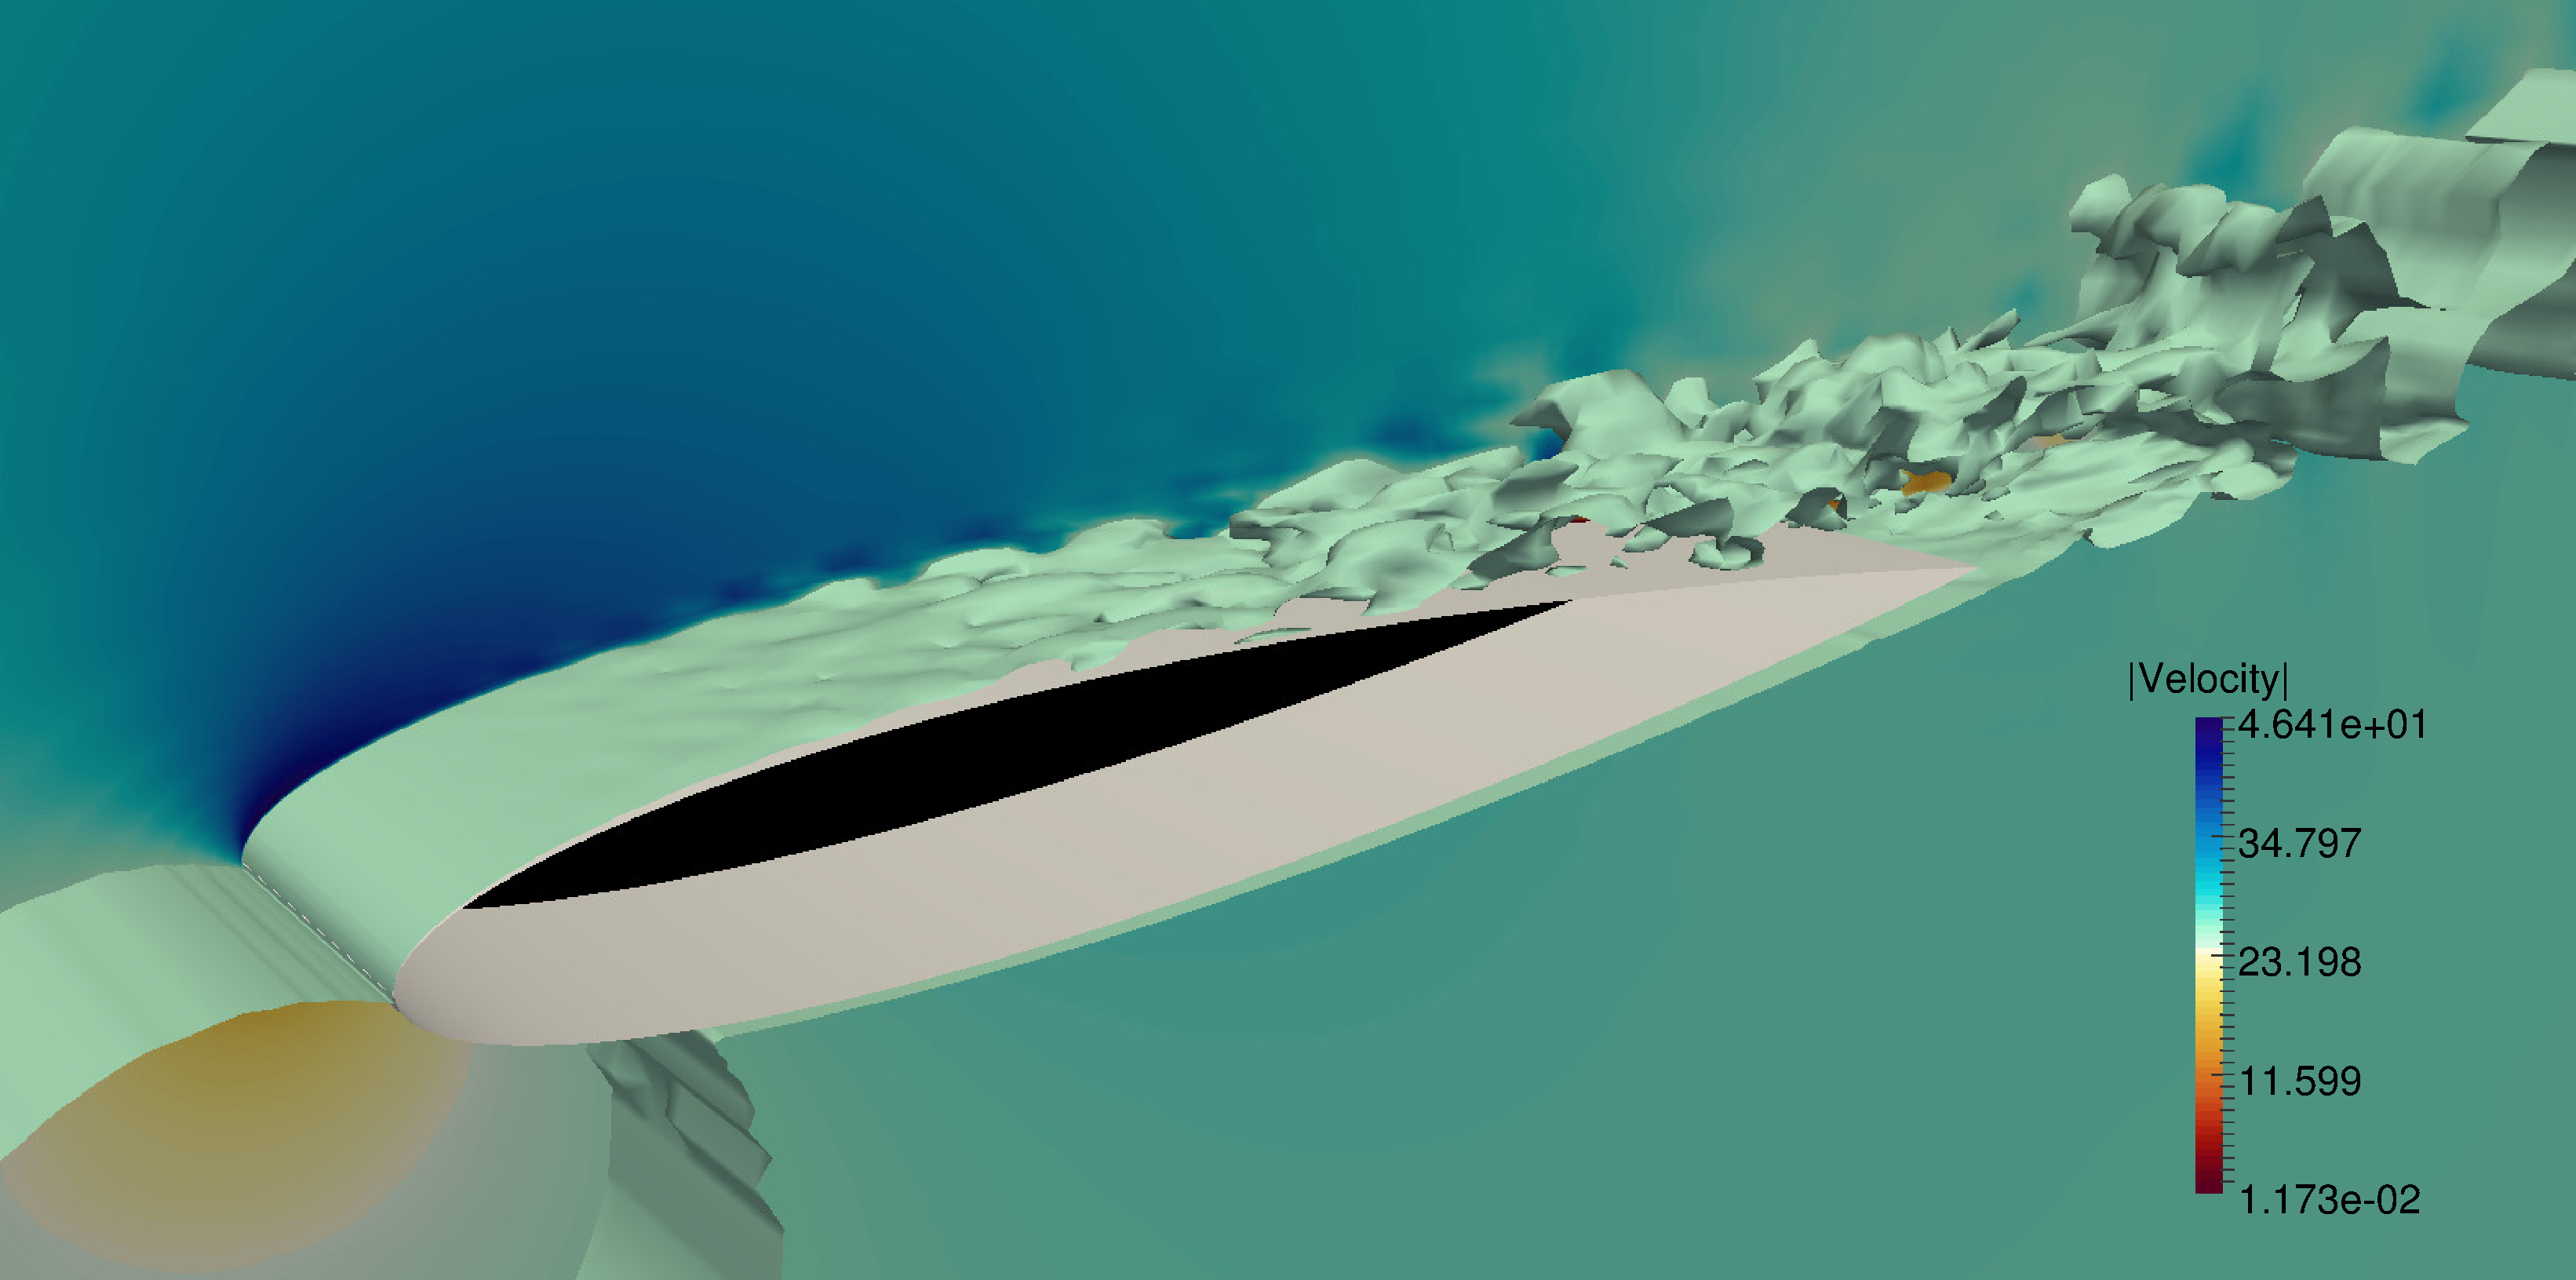
\includegraphics[width=0.9\textwidth]{Figures/Chapter8/weak/velo_3d}
  \caption{Velocity isosurface for $ \|\u\|=25.0  $.}
  \label{fig-NACA_3D_velo}
\end{figure}

To study the structures that arise in the turbulent flow we use the $Q$-criterion defined as $ Q=\frac{1}{2}(|\omega|^2-|\boldsymbol{\varepsilon}(\u)|^2) $, being $ \omega $ the vorticity and $ \boldsymbol{\varepsilon} $ the strain rate tensor. The isosurface of $ Q=5\cdot 10^5$ is depicted in \Fig{NACA_3D_Q}, where we can see the generation of 2D coherent vortices that break up near the maximum thickness point, turning into hairpin vortices. Similar results are obtained in \cite{Kojima}, where a much finner mesh is used to solve the same problem.
\begin{figure}[h!]
  \centering
  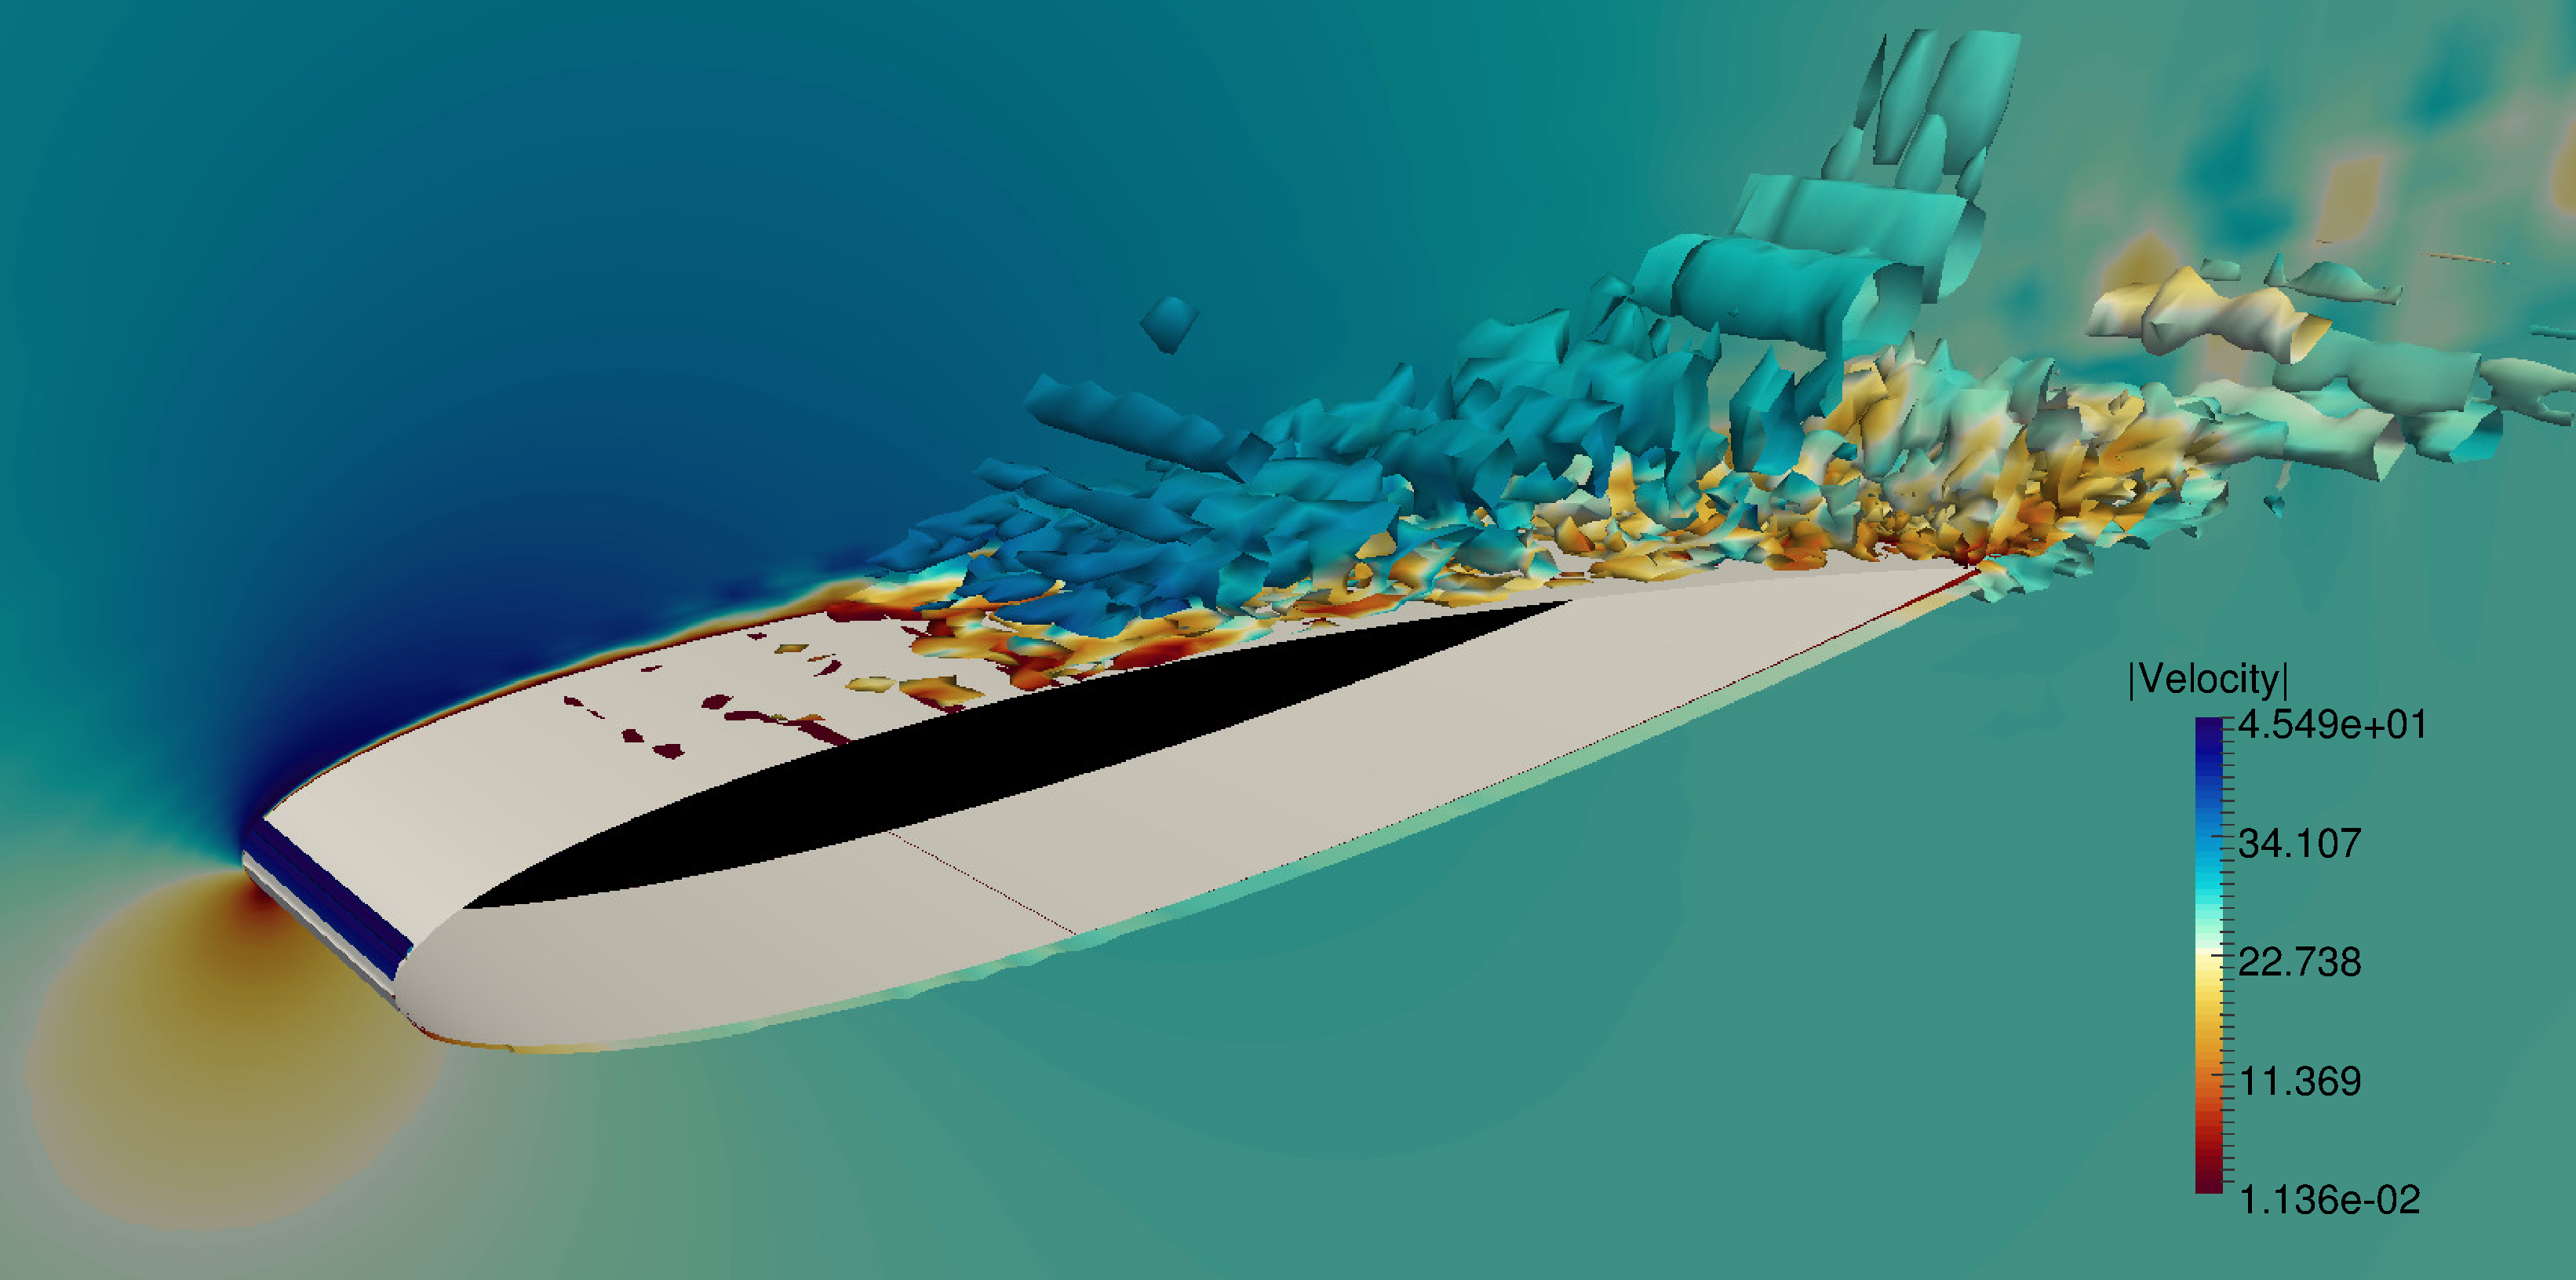
\includegraphics[width=0.9\textwidth]{Figures/Chapter8/weak/Q_criterion_3d}
  \caption{Q-criterion isosurface for $ Q=5\cdot10^5 $ and colored by velocity magnitude.}
  \label{fig-NACA_3D_Q}
\end{figure}
In \Fig{NACA_3D_Q_top} we present a top view of the $ Q=5\cdot 10^5 $ isosurface. There, we can see the position of the first 2D coherent vortex, located at $ x/c=0.37 $. This result is similar to the obtained in \cite{Kojima}, where the first 2D vortex is located at $ x/c=0.41 $.
\begin{figure}[h!]
  \centering
  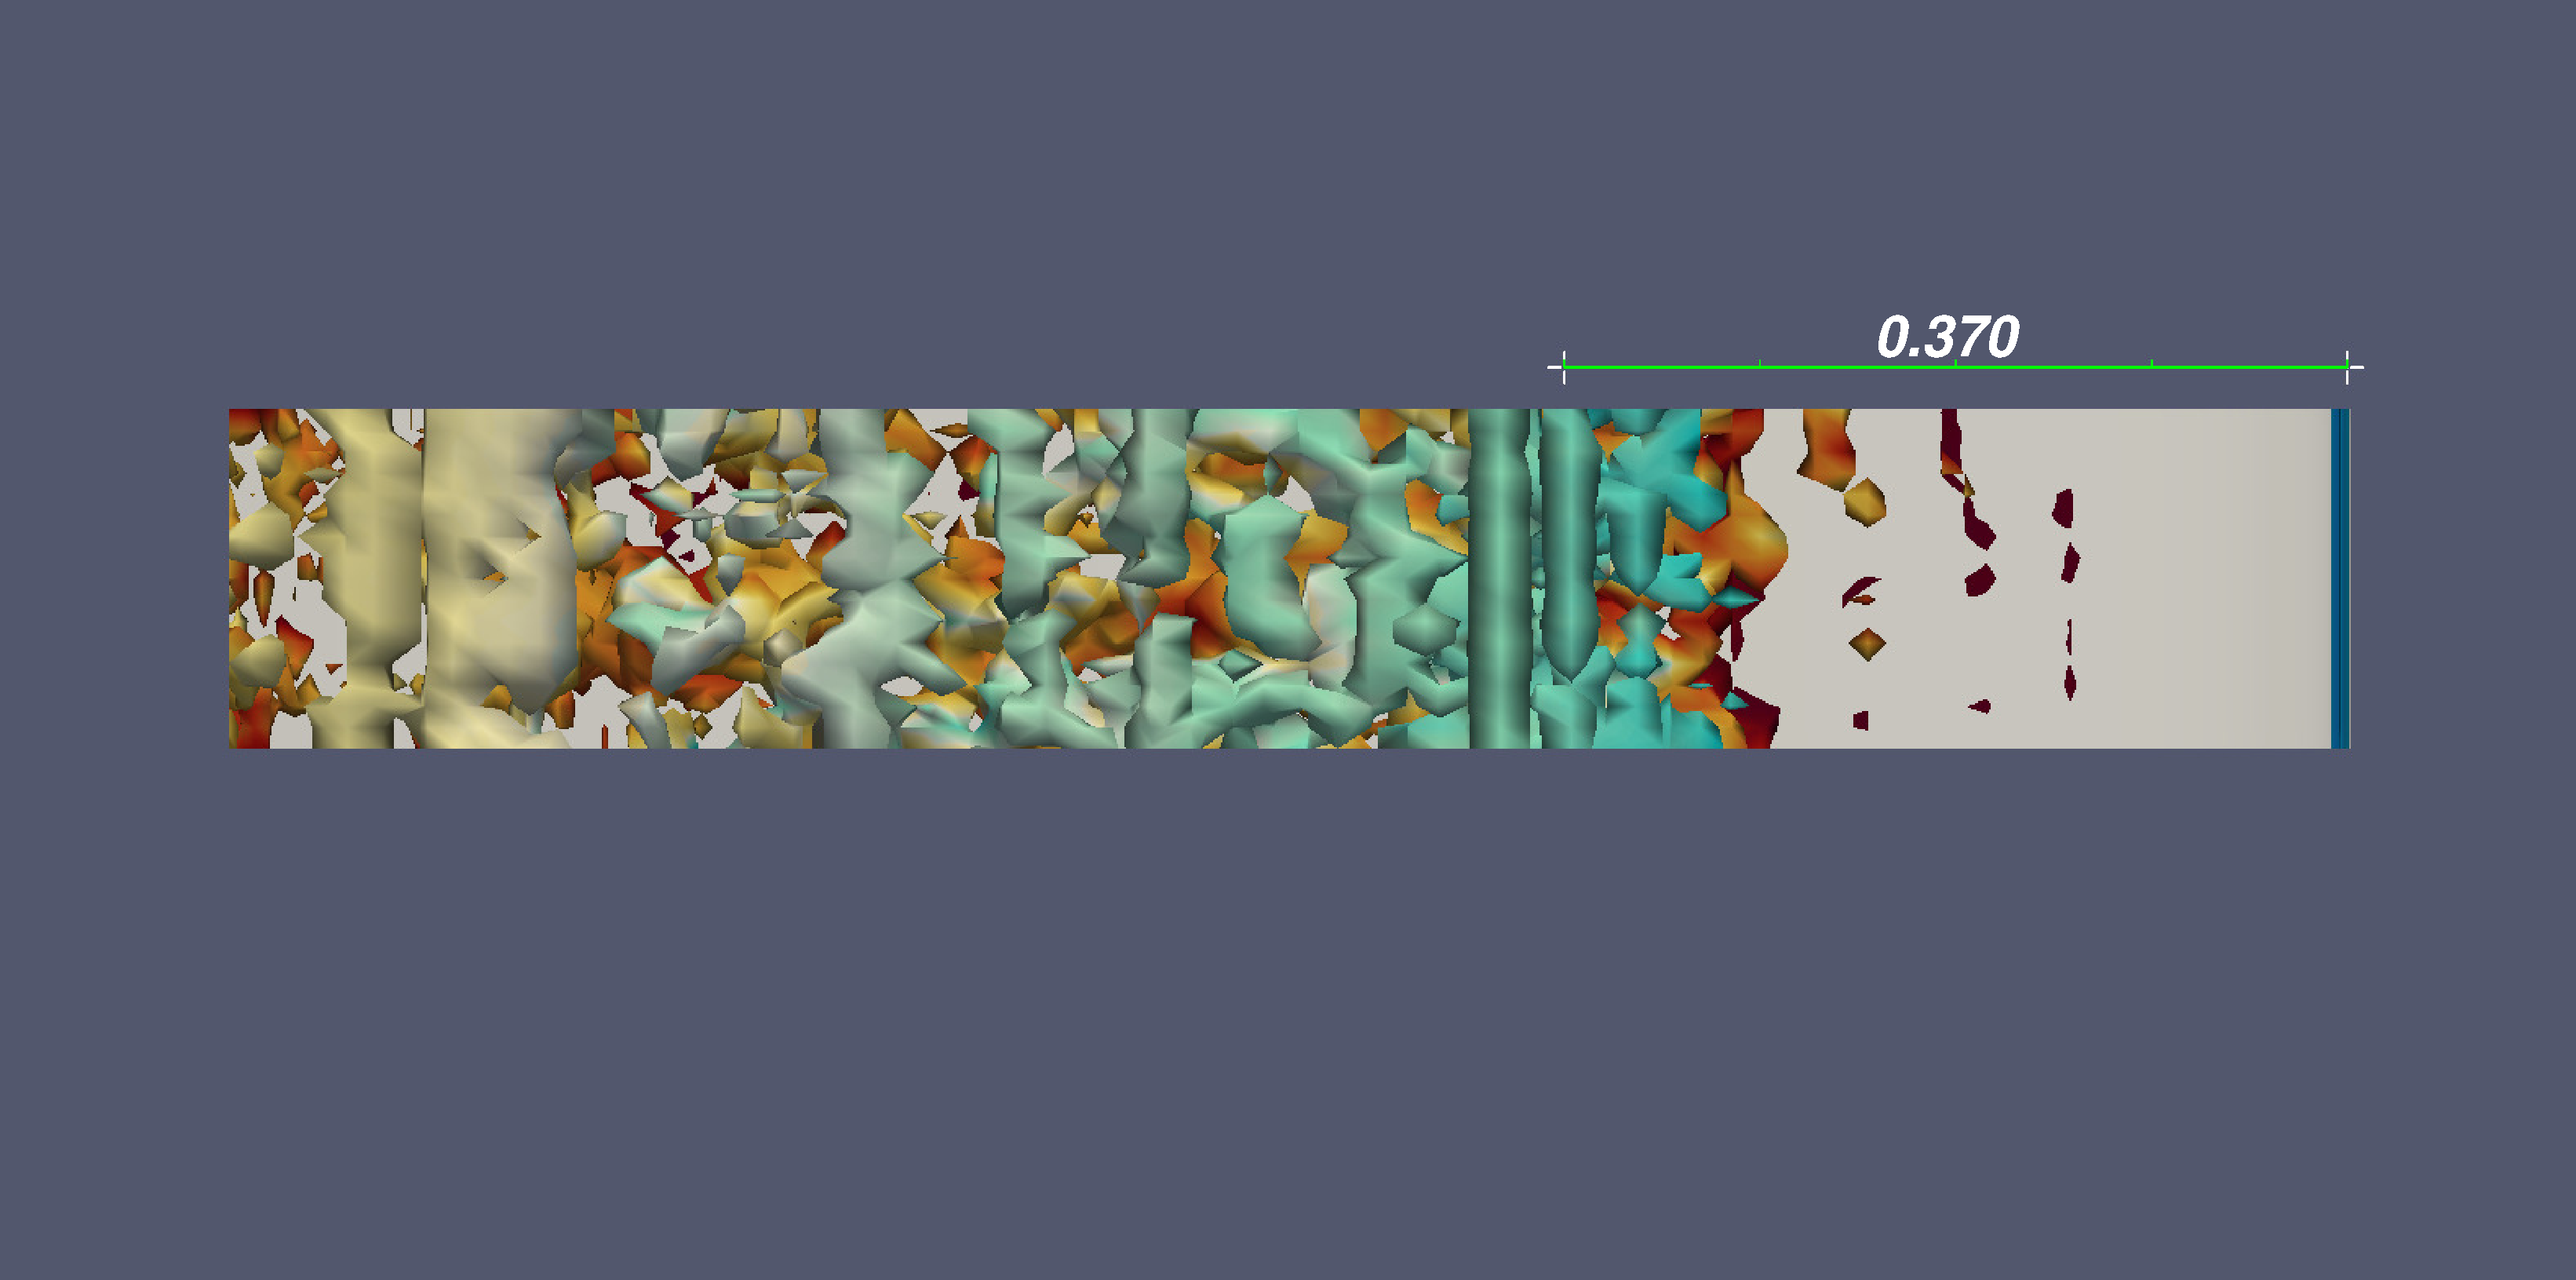
\includegraphics[width=0.9\textwidth,clip=true,trim=2cm 9cm 2cm 6cm]{Figures/Chapter8/weak/Q_criterion_rule}
  \caption{Top view of Q-criterion isosurface for $ Q=5\cdot10^5 $.}
  \label{fig-NACA_3D_Q_top}
\end{figure}

%\subsection{Aerodynamic coefficients}
%\subsubsection{Pressure Coefficient}
%\subsubsection{Drag coefficient}
%\subsubsection{Lift coefficient}
%
%
%
%The results obtained with the previous problem setting are compared against experimental data from Wadcock \cite{wadcock_investigation_1987} and Hastings et al. \cite{Hastings}. In order to have a better idea of the performance of our VMS approach we also compare against other LES models that have been used to solve the same problem. These are the Katenbach  et al. work \cite{kaltenbach_large-eddy_1995}, the data from Jansen \cite{jansen_stabilized_1999} and three different LES models proposed by Schmidt et al. in \cite{schmidt_assessment_????}.
%
%The pressure coefficient $C_p$ is shown in Fig. 
%%\begin{figure}[h!]
%%  \centering
%%  \subfigure[$C_p$ compared with experimental data]{\label{fig-NACA_cp_glob}\includegraphics[width=0.49\textwidth]{Figures/NACA/cp}}
%%  \subfigure[$C_p$ close up view compared with experimental data and other LES models]{\label{fig-NACA_cp_close}\includegraphics[width=0.49\textwidth]{Figures/NACA/cp_close}}
%%  \caption{Pressure coefficient $C_p$.}
%%  \label{fig-NACA_cp}
%%\end{figure}


%\begin{figure}[h!]
%  \centering
%  \subfigure[$x/c=0.529$]{\label{fig-NACA_profile1}\includegraphics[width=0.32\textwidth,clip=true,trim=3.5cm 0cm 3.5cm 0cm]{Figures/NACA/profile1}}
%  \subfigure[$x/c=0.815$]{\label{fig-NACA_profile2}\includegraphics[width=0.32\textwidth,clip=true,trim=3.5cm 0cm 3.5cm 0cm]{Figures/NACA/profile2}}
%  \subfigure[$x/c=0.952$]{\label{fig-NACA_profile3}\includegraphics[width=0.32\textwidth,clip=true,trim=3.5cm 0cm 3.5cm 0cm]{Figures/NACA/profile3}}
%  \caption{Mean streamwise velocity profiles normalized by $U_\infty$.}
%  \label{fig-NACA_cp}
%\end{figure}

\section{Conclusions}
\label{sec-C8_conclusions}
In this chapter we have tested the behavior of the SVMS method with weak boundary conditions based on a wall-law model for the simulation of turbulent flows around an airfoil. 

Considering weak boundary conditions when coarse meshes are used have been demonstrated to be necesary when the mesh size at the wall does not allow to capture properly the boundary layer. Furthermore, the weak imposition of the wall-normal component have been succesfully used in this test, avoiding the complex techniques that are required for the strong imposition of only the normal component on curvilinean geometries.

The effect of the algorithmic constatns $ c_c $ and $ \beta $ have been assessed for this test, concluding that, as noted in previous turbulent tests, the $ c_c $ constant has a clear effect on the solution. This phenomena have been studied in previous chapters, where the dependency of the solution on the $ c_c $ value have been related to the fact that the grad-div stabilization term is highly important when using inf-sup stable elements.



